\documentclass[12pt,a4paper]{article}
\usepackage{manual}
\usepackage{array}
\usepackage{longtable}

\newcommand\largeshot{0.7}
\newcommand\smallshot{0.5}


\renewcommand{\topfraction}{0.85}
\renewcommand{\textfraction}{0.1}

\begin{document}

\thispagestyle{empty}

\begin{center}

{\fontsize{32pt}{36pt}\selectfont Rubato Composer}

\vspace{20pt}

{\fontsize{20pt}{24pt}\selectfont User's Manual}

\vspace{28pt}

{\fontsize{14pt}{18pt}{\so{G�RARD MILMEISTER}}}

\vspace{48pt}

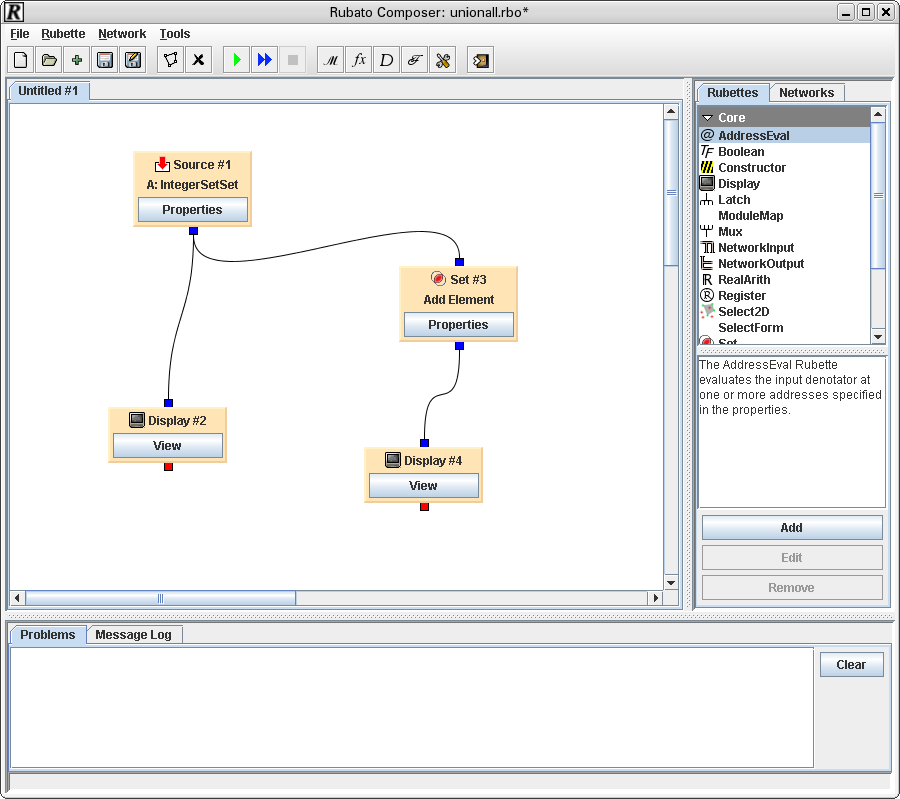
\includegraphics[width=0.8\linewidth]{composer}

\vfill

{\fontsize{14pt}{18pt}{\so{MARCH 2006}}}

\vspace{60pt}

\end{center}


\clearpage

\thispagestyle{empty}

\tableofcontents

\clearpage

\section{Introduction}
\label{manual:sec:introduction}

\composer{} GUI is part of the \composer{} software environment. It is the part that
offers a graphical interface to the less programming oriented user.  This manual offers a
complete description of the interactive elements of \composer{} as well as some technical
background including a tutorial guide to developing plug-ins and rubettes. The theoretical
foundations of denotator theory are not further discussed, some rudimentary familiarity is
presupposed.


\section{Concepts}
\label{manual:sec:concepts}

\composer{} uses elements from visual programming such as components and data-flow
links. The components are called \emph{rubettes} and are linked together and grouped in
\emph{networks}.


\subsection{\composer{}'s World of Objects}
\label{manual:sec:objects}

From an abstract point of view, \composer{} is an environment for creating and
manipulating objects. Therefore it is important to know the world of objects represented
within \composer. Each object may be stored under a name in a global system repository.
The namespaces for the kinds of objects are disjoint.
\begin{basedescript}{%
    \labelsep=0em%
    \desclabelwidth{6em}%
    \desclabelstyle{\nextlinelabel}%
    \renewcommand{\makelabel}[1]{\emph{#1}:}%
}
\item[Modules] Mathematical modules are the fundamental data types. They include
  integers, reals, vector spaces, etc.
\item[Module elements] Elements of modules are integers, reals, vectors, etc.
\item[Module morphisms] Functions between modules are called morphisms. They include
  affine morphisms, embeddings, etc.
\item[Forms] Forms constitute the general ``types'' of denotator theory. A form has an
  intrinsic non-empty name and \emph{must} be registered with this name in the system
  repository.
\item[Denotators] Denotators are the most general objects. A denotator may be
  anonymous or it may have an intrinsic name. A denotator with a non-empty name can be
  stored under this name in the system repository.
\item[Rubettes] A rubette instance is a computational entity, which works on denotators
  (see also \autoref{manual:subsec:rubetteconcept}). Rubette instances exist only within
  networks.
\item[Networks] Rubettes are placed and interconnected in networks to create data flow
  schemes.
\end{basedescript}

A \composer{} \emph{project} is an \emph{environment} consisting of a collection of
objects of above kinds. A project can be saved to disk in a file with extension
\textscreen{.rbo}. Thus a project file contains a list of definitions, where a
\emph{definition} is an assignment of a name to an object, such as a form to its intrinsic
name, a network to its name given during its creation or a module morphism that has been
assigned a name, etc. Saving a project into a file and reading it back has the effect of
restoring the environment. Be aware, however, that only objects that have been bound to a
name, and objects that these objects recursively depend on, are saved. Normal usage of
\composer{} does not produce non-transient dangling objects, i.e., objects that should be
saved, but are not.


\subsection{Rubettes}
\label{manual:subsec:rubetteconcept}

A rubette is a computational entity consisting of several inputs (including none), several
outputs (including none) and a computational core that computes outputs from inputs. In
general a rubette may provide a visual interface, of which there are two types:
\begin{enumerate}
\item Properties: This consists usually of a dialog that presents the UI elements for
  controlling the exact behavior of a rubette. In other words, here the fundamental
  parameters may be tweaked.
\item View: This window produces an audiovisual representation of the informational
  content of the rubette. For example, a rubette may show a musical score as a piano roll,
  similar to MIDI sequencer software. It may also allow playing the score through the
  local soundsystem or through connected MIDI hardware.
\end{enumerate}
Examples of these will be shown in \autoref{manual:sec:corerubettes} where all core rubettes are
described.

There are no constraints on the type of computation that a rubette embodies.  It may be a
simple mathematical calculation, but can also generate graphics or audio data, for example
as a MIDI player. However, it cannot be assumed that a rubette runs in real-time.

\setlength{\unitlength}{1mm}%
\begin{figure}[hbt]
  \centering
  \begin{picture}(30,25)(0,0)
    \put(0,0){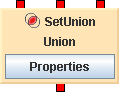
\includegraphics[width=3cm]{rubette}}
    % 
    \put(-9,21.2){\rightbox{Inputs}}
    \put(-7,22.2){\vector(1,0){10}} 
    % 
    \put(-9,17){\rightbox{Icon}}
    \put(-7,18){\vector(1,0){12}}
    % 
    \put(-9,5.3){\rightbox{Properties button}}
    \put(-7,6.3){\vector(1,0){8}}
    % 
    \put(39,17){Rubette instance name}
    \put(38,18){\vector(-1,0){12}}
    % 
    \put(39,11.7){Information text}
    \put(38,12.7){\vector(-1,0){17}}
    % 
    \put(39,0){Output}
    \put(38,1){\vector(-1,0){19}}
  \end{picture}
  \caption{Graphical representation of a rubette.}
  \label{manual:fig:rubette}
\end{figure}

\Autoref{manual:fig:rubette} shows what a rubette looks like as a manipulable object in
\composer. This is a simple rubette that takes several input denotators of type
\emph{power} (i.e., sets) and produces a result that is a set-theoretic function of its
inputs. The \emph{input} connectors (three of them in this case) are always on top, the
\emph{output} connectors (one in this case) at the bottom. Connectors are colored blue
when connected and red when not (this is seen in \autoref{manual:fig:network}).  An
optional \emph{icon} indicates the rubette type. The \emph{instance} name is a string that
can be assigned by the user to this rubette instance.  By default a new instance has a
name derived from the name of the rubette (\emph{SetOp} in this case) with a number
appended. The \emph{SetOp} rubette has a properties dialog that can be opened by clicking
the \emph{Properties button}. If a rubette has a view, then a second button for opening
the view would appear. Generally a rubette can be customized for the operation it
performs. In this case, operations include set union and intersection. A rubette may show
some information about its currently configured operation by specifying an
\emph{information text}.  For example, if the user changed the operation to intersection
in the properties dialog, the information text would display ``Intersection'' instead of
``Union''.


\subsection{Networks}
\label{manual:subsec:networkconcept}

\composer{} manages any number of networks, organized in a tabbed panel. A network is a
canvas, whereunto rubette instances are placed and connected. A network is just a
data flow diagram, similar to other visual programming tools. \Autoref{manual:fig:network} shows an
example of such a network: it contains four rubettes, named \emph{Source \#{1}}, \emph{Display \#{2}},
\emph{Set \#{3}} and \emph{Display \#{4}}.%
\begin{figure}[hbt]
  \centering
  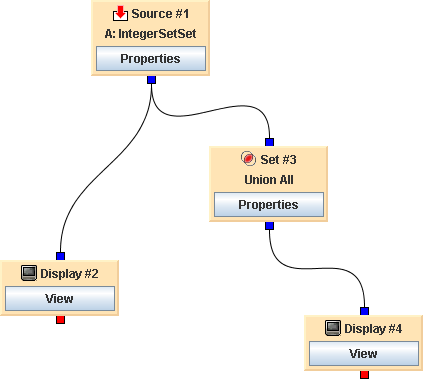
\includegraphics[scale=\largeshot]{network}
  \caption{Graphical representation of a network.}
  \label{manual:fig:network}
\end{figure}

Links are dragged from an output connector of a rubette to an input connector of another
rubette, or vice versa. Several links can start from one output connector, but at most one
link can enter an input connector. It is however possible to connect several inputs to one
input connector by routing them first through a multiplexer rubette. It is currently not
allowed to create directed cycles when building a network.

To perform the computation embodied by an network, it is \emph{executed}, or \emph{run}.
When execution is requested, the scheduler must determine in what order the rubettes are
run, since rubette inputs depend on outputs of other rubettes. To this end a topological
sort is done, and rubettes are run according to the resulting linear order. In the example
from \autoref{manual:fig:network}, the order would be \emph{Source \#{1}} $\prec$
\emph{Display \#{2}} $\prec$ \emph{Set \#{3}} $\prec$ \emph{Display \#{4}}, where the
preference of \emph{Display \#{2}} over \emph{Set \#{3}} is purely dependent on the
implementation and should be regarded as random. This mode of execution is known as
\emph{complete run}, since every rubette is scheduled. Another mode is \emph{continuous
  run}. Here the network is executed as soon as a rubette's configuration has been changed
by the user. The topological sort only considers the modified rubette and its dependents,
and only these are submitted to the scheduler for a partial run. This mode is suitable for
a more interactive use of \composer{}, since any manipulation of a rubette will
immediately result in updated views of depending rubettes.

Multiple networks are independent. However, a network may be packaged in a macro rubette
and can then be used as a regular rubette for building other networks. Of course, a
network may generate a denotator and register it globally under a name. This named
denotator can then be accessed from another rubette.


\subsection{Macro Rubettes}
\label{manual:subsec:macrorubette}

A network may itself exhibit the behavior of a rubette. To accomplish this, all elements
that define a rubette must be present. First, the computational part is assumed by the
network configuration. Then, the inputs and outputs are defined by putting rubettes of
types \emph{MacroInput} and \emph{MacroOutput}, respectively, into the network. The
\emph{MacroInput} rubette takes the place of the rubette inputs (1 to 8). Its output
connectors are the inputs to the macro rubette. The \emph{MacroOutput} rubette stands for
the rubette outputs (1 to 8), its input connectors will show up as outputs of the macro
rubette. At most one of each may be present. No \emph{MacroInput} rubette means no input
at all, similarly for \emph{MacroOutput}. Such a network is then packaged into a
\emph{MacroRubette} using a command available from the popup menu (right mouse button). At
this occasion, a name and a description can be specified. From then on, this macro rubette
is available for inclusion in other networks.

When an instance of a macro rubette is placed in a network, a complete copy of the macro
network is included, whence the name \emph{macro}. Two instances of a macro rubette are
completely independent. The network implementing the macro instance can be opened and
modified like a normal network. However, changes will be reflected in the instance, and
\emph{MacroInput} and \emph{MacroOutput} rubettes can neither be modified, removed, or
added anymore. Closing a macro network just closes the window, the macro network itself is
not deleted.


\subsection{Tools}
\label{manual:subsec:toolsconcept}

Apart from the central features of networks and rubettes, \composer{} provides extensive
tools for creating and manipulating the fundamental types of objects: modules, elements of
modules, module morphisms, forms and denotators.


\section{Using \composer}
\label{manual:sec:usingcomposer}

This section describes the usage of the graphical interface.


\subsection{Starting up}
\label{manual:subsec:startingup}

\composer{} and the \rubato{} framework are implemented in pure Java.  At least version
1.5 is required. The user interface is based on Swing, therefore independent
implementations like GCJ do not work yet. Hopefully this will change in a not so far
future. There are currently no plans for a reimplementation with an alternative toolkit
such as SWT.

Currently \composer{} is started by executing the JAR archive named
\textscreen{rubato.jar} or \textscreen{rubato-}\textit{DATE}\textscreen{.jar}, where
\textit{DATE} is the version of the distribution. On most platforms this is done by
executing the command line \textscreen{java -jar rubato.jar}. There are currently no
platform-specific mechanisms for starting the application.


\subsection{General Usage}
\label{manual:subsec:generalusage}

As a Swing application, the basic graphical elements of \composer{}, such as file dialogs,
follow the guidelines of Swing on the specific platforms. Many operations are available
from the toolbar as well as from the menubar. Others can be directly invoked using
keyboard shortcuts. These shortcuts are summarized in \autoref{manual:sec:shortcuts}.


\subsection{Main Window}
\label{manual:subsec:mainwindow}

\begin{figure}[hbt]
  \small
  \centering
  \begin{picture}(80,75)(0,0)
    \put(0,0){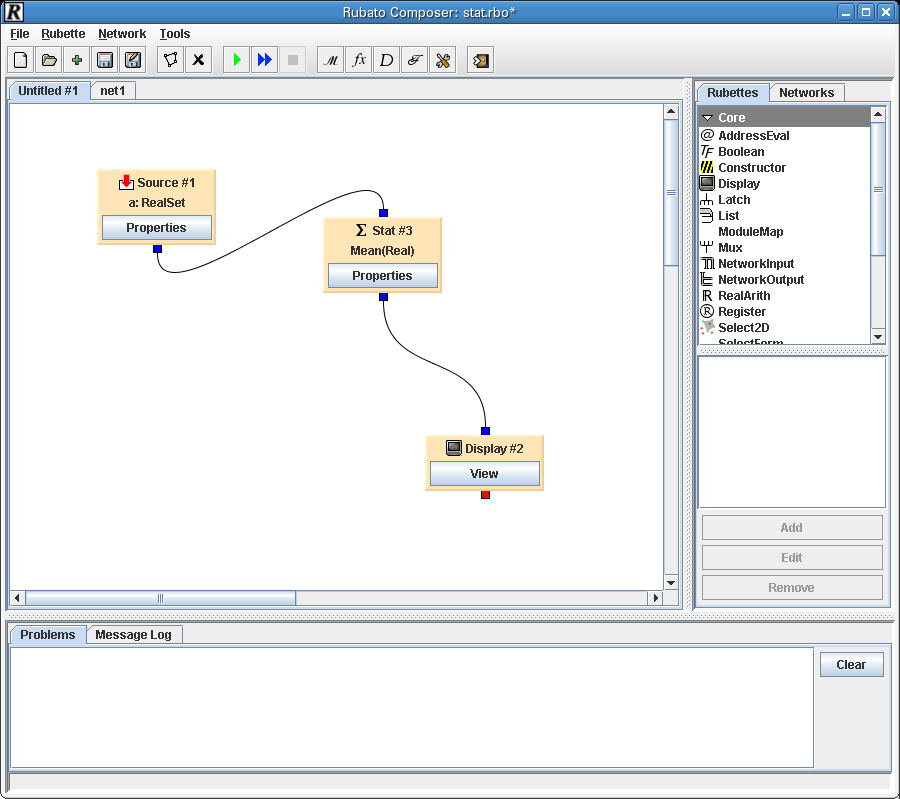
\includegraphics[width=8cm]{mainwindow}}
    % 
    \put(20,73){\rightbox{Main menu}}
    \put(13.5,72.2){\vector(0,-1){4}}
    % 
    \put(-3,65){\rightbox{Toolbar}}
    \put(-2,66){\vector(1,0){6}}
    % 
    \put(-3,36){\rightbox{Network}}
    \put(-2,37){\vector(1,0){8}}
    % 
    \put(-3,10){\rightbox{Message log}}
    \put(-2,11){\line(1,0){13}}
    \put(11,11){\vector(0,1){3}}
    \put(-3,6){\rightbox{Problem log}}
    \put(-2,7){\vector(1,0){8}}
    % 
    \put(-3,0.4){\rightbox{Statusbar}}
    \put(-2,1.4){\vector(1,0){8}}
    % 
    \put(84,50){Rubette panel}
    \put(83,51){\vector(-1,0){8}}
    \put(81.5,51){\line(0,-1){20}}
    \put(81.5,31){\vector(-1,0){6.5}}
    % 
    \put(84,62){Network list}
    \put(83,63){\vector(-1,0){8.5}}
  \end{picture}
  \caption{Main window.}
  \label{manual:fig:mainwindow}
\end{figure}

\emph{Main window.} The overall layout of the main window is shown in
\autoref{manual:fig:mainwindow}. Apart from the main menu and the toolbar, there are three areas
for importance. The largest part is taken up by the tabbed panel of networks, where each
tab is occupied by one network.

\emph{Right panel.} The right panel consists of two tabs, the \emph{rubette panel} and the
\emph{network list}. The rubette panel contains all types of rubettes currently available
to the application. Rubettes are grouped under various headings. The heading \emph{Core}
is always present and contains the built-in core rubettes (see
\autoref{manual:sec:corerubettes}). By clicking on a heading the rubettes in the group are shown or
hidden. A double click on a rubette will put an instance of its type into the currently
visible network (if there is no network at all, nothing happens). Alternatively a rubette
may be selected and then dragged onto the network. Below the list of rubettes, a text
areas display a description of the selected rubettes. The \textscreen{Add} button performs
the same thing as a double-click. The \textscreen{Edit} and \textscreen{Remove} buttons
are active only when a macro rubette is selected.

The other tab contains the network panel. It is simply a list of all existing networks. A
mouse click on a network name will make this network visible.

\emph{Bottom panel.} The bottom panel is reserved for the display of information. It has
two views, the \emph{problem log} and the \emph{message log}. The message log
(\autoref{manual:fig:messagelog}) records general activity, such as adding rubettes, loading and
saving, indicating any errors that occurred.
\begin{figure}[hbt]%
  \centering
  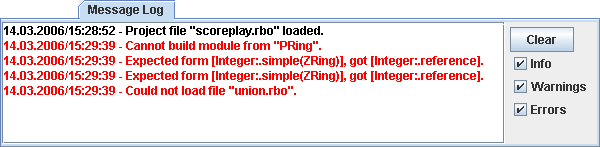
\includegraphics[scale=\smallshot]{messagelog}
  \caption{Message log tab.}
  \label{manual:fig:messagelog}
\end{figure}
Messages are of three types, info for informational messages such as indications of
performed actions (in black), warnings for undesirable but non-fatal occurrences (in
\textcolor[rgb]{0.84,0.46,0.03}{orange}) and errors indicating unrecoverable failures such
as unsuccessful loading of files (in \textcolor{red}{red}). The checkboxes at the right
side of the log window determine what types should be displayed. The \textscreen{Clear}
button will erase the list. All generated messages are also shown at the bottom-most
statusbar for a few seconds.

The problem log lists those errors that occur during the execution of a network. It is
cleared at the beginning of each run. Since errors are always relative to a rubette, it is
possible to a highlight the responsible rubette by clicking on an error message line. The
highlighted rubette is surrounded by a thin red frame.
\begin{figure}[hbt]%
  \centering
  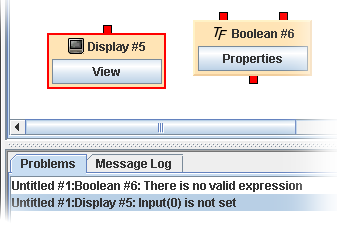
\includegraphics[scale=\largeshot]{problemlog}
  \caption{Problem log tab. The second line indicates that there is no input on
    the red-framed rubette \emph{Display \#5}.}
  \label{manual:fig:problemlog}
\end{figure}


\subsection{Main Menu and Toolbar}
\label{manual:subsec:menutoolbar}

\begin{basedescript}{%
    \labelsep=0em%
    \desclabelwidth{8em}%
    \desclabelstyle{\nextlinelabel}%
    \renewcommand{\makelabel}[1]{\textscreen{#1}}%
}
\item[File\arrow New] \emph{Create a new project}. The environment is reset to the fresh state
  as at startup, i.e., all objects, except for the built-ins, are deleted.
\item[File\arrow Open\ldots] \emph{Open an existing project}.  A rubato project file
  (extension \textscreen{.rbo}) is loaded into the environment. All previously created
  objects, except for the built-ins, are deleted.
\item[File\arrow Add Definitions\ldots] \emph{Add definitions from an existing
    \textscreen{.rbo} file}.  A rubato project file (extension \textscreen{.rbo}) is
  loaded into the environment. In contrast to \textscreen{File\arrow Open}, the
  environment is not cleared, but the definitions from the file are merged into it.
\item[File\arrow Revert] \emph{Revert project to a saved state}. If the current project
  has been saved at least once, reload it from the file with clearing the environment
  first.
\item[File\arrow Save] \emph{Save project}. If the current project has been saved at least
  once, save it under its given name, otherwise a filename (with \textscreen{.rbo} extension)
  is requested.
\item[File\arrow Save As\ldots] \emph{Save project under a new name}. A file name is
  requested regardless whether the project has already been saved once or not.
\item[File\arrow Recent Files] \emph{Open recently used project}. This submenu contains
  recently opened projects. The list is saved when the program exits and can be cleared
  using the \textscreen{Clear} entry in the submenu.
\item[File\arrow Quit] \emph{Leave \composer}. The application is
  closed. If there are unsaved changes, the user is asked if he wants to save.
\item[Rubette\arrow Add Rubette] \emph{Create new rubette instance}. A new instance of
  the rubette selected in the rubette list is added to the current network if there is
  any, otherwise nothing is done.
\item[Network\arrow New network] \emph{Create new network}. A new, empty network is
  created and displayed as a new tab. It receives a default name of the form
  ``\incode{Network \#}$n$'' where $n$ is a serial number.
\item[Network\arrow Close network] \emph{Close visible network}. The current, visible
  network is deleted. If the currently visible network is the representation of a macro
  rubette, it is simply removed from view.
\item[Network\arrow Run] \emph{Run visible network}. The execution of the current, visible
  network is started. This menu item is disabled if there is already an execution in progress.
\item[Network\arrow Stop] \emph{Stop network execution}. The current execution is
  stopped. This menu item is disabled if there is no execution in progress.
\item[Tools\arrow Module Builder] \emph{Open module builder tool}. The module builder is
  shown. There is always at most one module builder window.
\item[Tools\arrow Module Morphism Builder] \emph{Open module morphism builder tool}. The
  module morphism builder is shown. There is always at most one module morphism builder
  window.
\item[Tools\arrow Denotator Builder] \emph{Open denotator builder tool}. The denotator
  builder is shown. There is always at most one denotator builder window.
\item[Tools\arrow Form Builder] \emph{Open form builder tool}. The form builder is
  shown. There is always at most one form builder window.
\item[Tools\arrow Object Browser] \emph{Open object browser tool}. The object browser is
  shown. There is always at most one object browser window.  
\item[Tools\arrow Scheme Interaction] \emph{Open Scheme interaction tool}. The Scheme
  interaction dialog is shown. There is always at most one Scheme dialog window.
\item[Tools\arrow Scheme Editor] \emph{Open Scheme code editor}. The Scheme code
  editor is shown. There is always at most one Scheme editor window.
\item[Tools\arrow Preferences] \emph{Change settings}. The preferences dialog is shown
  where settings that affect the overall behavior of \composer{} can be changed
  (see~\autoref{manual:subsec:prefs}).
\end{basedescript}


\subsection{Network}
\label{manual:subsec:network}

The multiple networks are laid out as several tabs in the middle of the application
window. New networks can be created using \textscreen{Network\arrow New Network} or the
\raisebox{-1pt}{
\includegraphics[scale=0.7]{newneticon}} button. Networks can be removed
again with \textscreen{Network\arrow Close Network}, the
\raisebox{-2pt}{
\includegraphics[scale=0.7]{closeicon}} button or \textscreen{Network.Popup\arrow
  Close network}. The last refers to the popup menu that is activated by clicking the
right mouse button in a network window. All operations in the popup menu are relative to
the currently visible network. The network popup menu is shown in
\autoref{manual:fig:networkpopup}.
\begin{figure}[htb]%
  \centering
  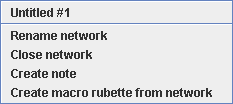
\includegraphics[scale=\largeshot]{networkpopup}
  \caption{Network popup menu.}
  \label{manual:fig:networkpopup}
\end{figure}%
The first line in the menu shows the name of the network (the same name is shown as the
title of the tab). The command \textscreen{Network.Popup\arrow Rename network} will open a dialog
requesting the user to enter a new name for the network. When a network is created, it is assigned a name
of the form \emph{Untitled \#$n$}, where $n$ is a serial number.

An additional feature of networks are notes, which work like sticky notes
(\autoref{manual:fig:note}). 
\begin{figure}[htb]%
  \centering
  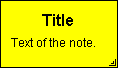
\includegraphics[scale=\largeshot]{note}
  \caption{Sticky note: the lower right handle can be used to resize the note.}
  \label{manual:fig:note}
\end{figure}%
They don't affect the computation of a network, but can be useful for adding information
and explanations.  A new note is created at the cursor position with
\textscreen{Network.Popup\arrow Create note}. Text can be entered into a note by clicking
on its contents. Notes can be resized, their background and foreground colors can be
changed and they can be given a title by activating its popup menu with a right mouse
click. Of course, notes can be removed again.

The procedure of adding rubettes and linking them together has already been discussed.
Rubettes can be dragged around on the network and have their own popup menu, which is
available by right-clicking whenever the pointer is over the rubette that is indicated by
a black border surrounding the rubette selected in this way. The first line of
\textscreen{Rubette.Popup} shows the name of the rubette, the same as is shown on the
rubette representation itself. The command \textscreen{Rubette.Popup\arrow Rename}
requests a new name from the user. A rubette is removed from the network by invoking
\textscreen{Rubette.Popup\arrow Remove}.  The command \textscreen{Rubette.Popup\arrow
  Duplicate} creates a copy of the selected rubette with a newly generated name. The
duplicate should have the same settings as the original.  However, what this exactly means
has to be specified by the developer of the rubette.  The \textscreen{Rubette.Popup\arrow
  Move To Front} and \textscreen{Rubette.Popup\arrow Move To Back} commands have the same
effect as similarly named operations in common graphics software.  The special operation
\textscreen{Rubette.Popup\arrow Pass Through} can be used to temporarily disable the
selected rubette. It is available only for rubettes with at least one input and at least
one output.  When this operation is toggled, the color of the rubette changes to
\textcolor[rgb]{1,0.5,0.31}{orange} and the execution of the rubette bypasses the proper
computational code and simply copies the first input to the first output, doing nothing
with the other inputs and outputs.

Several operations are available from the popup menu that opens when right-clicking on a
link. The command \textscreen{Link.Popup\arrow Remove Link} does the obvious thing. The
three remaining options, \textscreen{Link.Popup\arrow Diagonal},
\textscreen{Link.Popup\arrow Zigzag} as well as \textscreen{Link.Popup\arrow Curved} each
select one of the three ways of representing the link.

A network is run by invoking \textscreen{Network\arrow Run} or the button
\raisebox{-2pt}{
\includegraphics[scale=0.7]{runicon}}. A running network can be
interrupted with \textscreen{Network\arrow Stop} or
\raisebox{-2pt}{
\includegraphics[scale=0.7]{stopicon}}. The effectivity of this operation
depends at least in part on the behavior of the individual rubettes and how they react to
the stop event. The button \raisebox{-2pt}{
\includegraphics[scale=0.7]{runconticon}}
toggles the continuous run mode.


\subsection{Tools}
\label{manual:subsec:tools}

The functionality available from the \textscreen{Tools} menu can be regarded as an
interface to the system repository. Objects are created and registered under a specified
name in the repository. The dialogs corresponding to the various types of objects (except
forms) may also appear when such an object needs to be specified, for example in the
properties of a rubette. In this case, a name need not be given, since the object in
question is used immediately.


\subsubsection*{Module Builder}

Similarly to other builders, the interface changes dynamically depending on the selected
values. \Autoref{manual:fig:modulebuilder} shows the creation of the module
$(\mathbb{Z}[X]\times\mathbb{R})^3$.
\begin{figure}[htb]
  \centering
  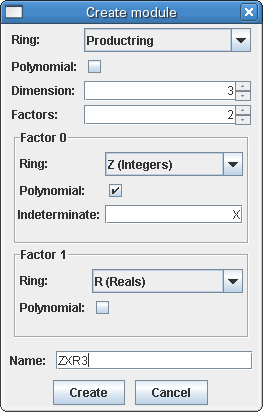
\includegraphics[scale=\smallshot]{modulebuilder}
  \caption{The module builder.}
  \label{manual:fig:modulebuilder}
\end{figure}
First the ring of the module is specified, in this case \textscreen{Productring} is
chosen, which requires further information. The checkbox below indicates whether it is a
ring of polynomials. Another element that is always present is the dimension of the free
module, here $3$. For a product ring, the number of factors is indicated and the factors of
the product have to be given. For each factor a module builder is recursively
inserted. The first factor, for example, is a ring of polynomials with indeterminate $X$
and coefficients in $\mathbb{Z}$. Finally a name must entered, here \textscreen{ZXR3},
before the module is created and registered with this name.


\subsubsection*{Module Morphism Builder}
\label{manual:subsubsec:morphbuilder}

The interface for creating module morphisms is probably the most extensive throughout
\composer{}. The reason is that morphisms come in many types and there are many ways to
specify them, even in the case of a single type.

As before, only some general hints are given, and a specific example is presented
(\autoref{manual:fig:morphbuilder}), since the interface is subject to extension.
\begin{figure}[htb]
  \centering
  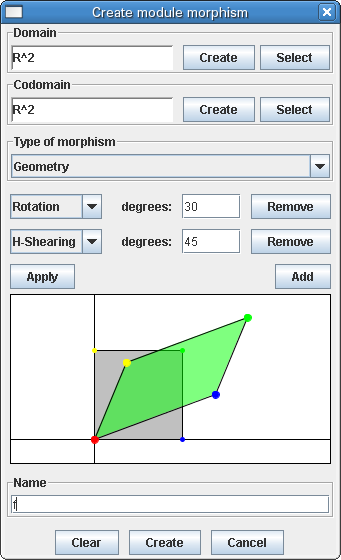
\includegraphics[scale=\smallshot]{morphbuilder}
  \caption{The module morphism builder.}
  \label{manual:fig:morphbuilder}
\end{figure}
Besides the name entry, the two module entries (see also \autoref{manual:subsubsec:modentry}) for
the domain and the codomain of the module morphism to be created are always present. The
builder may however be configured programmatically to fix one or both of the domain or
codomain, for example if a module morphism is required to have a given domain (i.e., the
domain is fixed) but an arbitrary codomain (i.e., the codomain must be specified). Finally,
the type of morphism must be selected. The list of available types depends of course on
the particular domain and codomain. \Autoref{manual:sec:modulemorphisms} contains an overview
of the currently available types.

In the example of \autoref{manual:fig:morphbuilder}, the morphism with name \textscreen{f}
is of the type $\mathbb{R}^2\to\mathbb{R}^2$. This is a transformation in the Euclidean
plane. The type is \textscreen{Geometry}, which allows the definition as composition of
geometric transformations. Here it is a rotation by $30^\circ$ followed by a horizontal
shearing by $45^\circ$. Transformations can be added and removed using the corresponding
buttons. After the button \textscreen{Apply} has been pressed, the resulting morphism is
created and its effect visualized on a unit square (vertexes are colored, otherwise
reflections might not be recognized as such).


\subsubsection*{Denotator Builder}
\label{manual:subsubsec:denobuilder}

Building denotators is less complicated than building morphisms, since there are only a
few types to consider: \Simple, \Limit, \Colimit, \Power{} and
\List. Generally the name and the form has to be specified. However in other
contexts the form may be programmatically fixed.

\Simple: The address type is required. If it is \textscreen{Null} the dialog accommodates
a module element entry. If it is \textscreen{Non-Null}, a module morphism must be selected with
codomain fixed to the module of the denotator form. In \autoref{manual:fig:simpledeno}, the
denotator to be created is given the name \textscreen{d} and should have form \emph{Real},
which has module $\mathbb{R}$.  The denotator is $\mathbb{Z}$-addressed and its morphism
is the embedding of $\mathbb{Z}$ into $\mathbb{R}$.
\begin{figure}[htb]
  \centering
  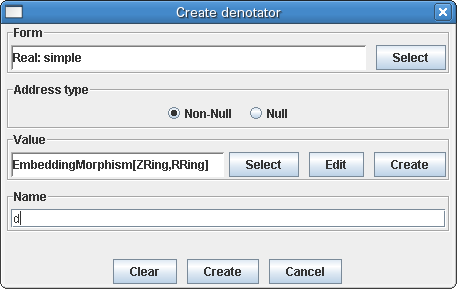
\includegraphics[scale=\smallshot]{simpledeno}
  \caption{\Simple{} denotator builder.}
  \label{manual:fig:simpledeno}
\end{figure}

\Limit: For a denotator of type \Limit, the coordinates must be specified.  In
\autoref{manual:fig:limcodeno}, the four coordinates for the denotator of form \emph{Note}
have the forms \emph{Onset}, \emph{Pitch}, \emph{Loudness} and \emph{Duration},
respectively. In this case the form also features labels for each of the coordinates indicated
in square brackets. The resulting denotator has the name \textscreen{n1} and is built from
the coordinates \textscreen{o1}, \textscreen{p1}, \textscreen{l1} and \textscreen{d1}.
\begin{figure}[htb]
  \centering
  \begin{tabular}{c}
    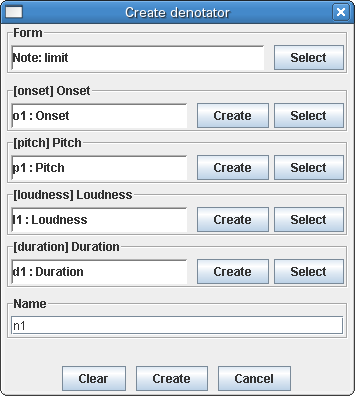
\includegraphics[scale=\smallshot]{limitdeno}
  \end{tabular}
  \begin{tabular}{c}
    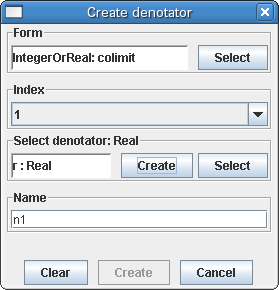
\includegraphics[scale=\smallshot]{colimitdeno}
  \end{tabular}
  \caption{\Limit{} (left) and \Colimit{} (right) denotator builder.}
  \label{manual:fig:limcodeno}
\end{figure}

\Colimit: A denotator of type \Colimit{} specifies exactly one coordinate. The index of
the cofactor must be given.

\Power: The elements of the set can be added to (buttons \textscreen{Add} and
\textscreen{Add New}) and removed from (button \textscreen{Remove}) the list. The
elements are shown in a compact representation, i.e., the name of an non-anonymous
denotator, or, otherwise, the address and form. Since the content of a denotator can be
very extensive, it is not included in the representation, but may be shown in the lower
text field by selecting the element.
\begin{figure}[htb]
  \centering
  \begin{tabular}{c}
    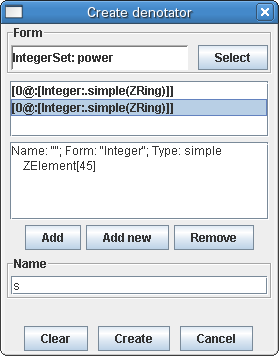
\includegraphics[scale=\smallshot]{powerdeno}
  \end{tabular}
  \begin{tabular}{c}
    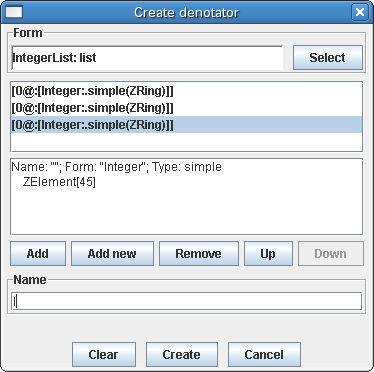
\includegraphics[scale=\smallshot]{listdeno}
  \end{tabular}
  \caption{\Power{} (left) and \List{} (right) denotator builder.}
  \label{manual:fig:powerdeno}
\end{figure}

\List: The interface for type \List{} is very similar to the \Power{}
interface. Since the order of the elements in a \List{} denotator is critical, two
further buttons (\textscreen{Up} and \textscreen{Down}) allow the (re)ordering of the
elements.


\subsubsection*{Form Builder}
\label{manual:subsubsec:formbuilder}

The interface of the form builder always features a selection box for the form type (the
fixed list consisting of \Simple, \Limit, \Colimit, \Power, and
\List) and the entry for the name. In contrast to denotators, forms \emph{must
  always} be given a name. The name entry box also checks whether the name is unique.
Invoking the form builder from the \textscreen{Tools} menu is the only way to create new
forms in the \composer{} GUI.

The interface for the \Simple{} type requires the entry of a module, whereas the
interfaces for types \Power{} and \List{} require the entry of the coordinate form.
\Autoref{manual:fig:powerform} shows the interface for creating \Power{} forms, the
interface for \List{} is the same.
\begin{figure}[htb]
  \centering
  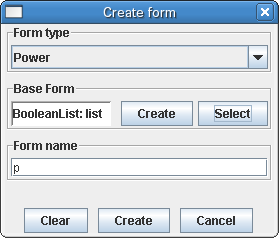
\includegraphics[scale=\smallshot]{powerform}
  \caption{\Limit{} form builder.}
  \label{manual:fig:powerform}
\end{figure}

The types \Limit{} and \Colimit{} have similar interfaces
(\autoref{manual:fig:limitform}).
\begin{figure}[htb]
  \centering
  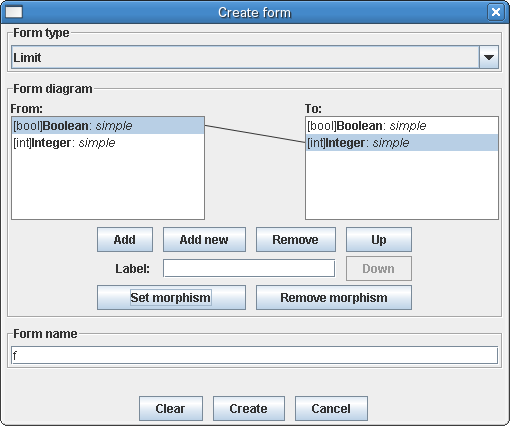
\includegraphics[scale=\smallshot]{limitform}
  \caption{\Limit{} form builder.}
  \label{manual:fig:limitform}
\end{figure}
The factor (resp. cofactor) forms are added to a list and can be reordered. The button
\textscreen{Add} allows the selection of a form from a list, the button \textscreen{Add
  New} invokes the form builder recursively. When a label is entered before a new form is
added, this label will be attached to the new factor (cofactor).

\emph{The following describes a feature not yet completely implemented.} The list of
factor (cofactor) forms is shown twice. When one form on the left and one on the right is
selected, a morphism between the two can be created using \textscreen{Set morphism}. This
is in fact the interface for creating non-trivial diagrams.


\subsubsection*{Object Browser}

The system-wide repository is a dictionary that associates names to objects of the types
module, element, module morphism, form and denotator. All forms must be registered in this
repository, for all other objects this is optional. The object browser
(\textscreen{Tools\arrow Object Browser}) presents a view of the repository. Whenever a
selected object can be edited, the \textscreen{Edit} button will open an editor to this
object.
\begin{figure}[htb]
  \centering
  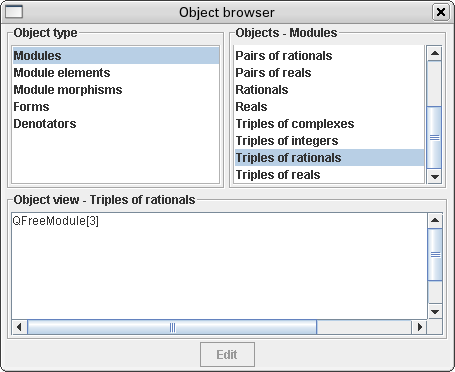
\includegraphics[scale=\smallshot]{browser}
  \caption{The object browser, a view of the repository.}
  \label{manual:fig:browser}
\end{figure}


\subsection{Scheme Tools}

\subsubsection*{Scheme Interaction}

The Scheme interaction dialog allows the evaluation of Scheme expressions in the global
Scheme environment. 

The top part of the dialog is the input area, where Scheme expression are entered. The
expressions in this area are evaluated by pressing \textkey{Ctrl-Enter}, and the result of
the evaluation is appended to the output area in the middle of the dialog. The keys
\textkey{Ctrl-Up} and \textkey{Ctrl-Down} navigate through a history of previous
expressions. Errors are shown in the bottom line.

The \textscreen{Stop} button interrupts a running evaluation, the \textscreen{Clear}
button blanks the output area and the \textscreen{Init} button resets the global Scheme
environment to the initial state.

\subsubsection*{Scheme Editor}

The Scheme editor allows to write Scheme code that can be evaluated in the global Scheme
environment. The code text is saved as part of the project.


\subsection{Preferences}
\label{manual:subsec:prefs}

The following settings are currently available:
\begin{basedescript}{%
    \labelsep=0em%
    \desclabelwidth{2em}%
    \desclabelstyle{\nextlinelabel}%
    \renewcommand{\makelabel}[1]{\textscreen{#1}}%
  }
\item[Default link type] Set to one of \incode{Line}, \incode{ZigZag} or \incode{Curve}
  determines what shape the links should be drawn in (default: \incode{Curve}), see
  \autoref{manual:fig:linktypes}.
  \begin{figure}[htb]
    \centering
    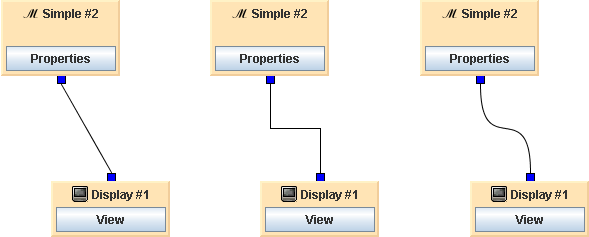
\includegraphics[scale=\smallshot]{links}
    \caption{Link types: Line (left), ZigZag (middle), Curve (right).}
    \label{manual:fig:linktypes}
  \end{figure}
\item[Save main window position and size] If set, leaving the application will save the
  last position and size of the main window. These are restored when the application is
  restarted (default: not set).
\item[Ask before leaving] If set, the user is asked when leaving the application and
  there are unsaved changes (default: set).
\item[Default Quantization] During conversion from reals to rationals, the generated
  denominators are always divisors of this integer.
\end{basedescript}


\subsection{Recurring User Interface Elements}
\label{manual:subsec:intelements}

Besides the usual Swing user interface elements, \composer{} makes use of some custom
elements that can be found throughout the system. These elements may be used by the
developer of rubettes, therefore the name of the class is indicated for easier reference.


\subsubsection*{Module Entry (\incode{JModuleEntry})}
\label{manual:subsubsec:modentry}

A module entry component (i.e., user interface element or widget) allows the user to
specify a module.  The left field shows the currently selected module, the button
\textscreen{Create} builds a new one, the button \textscreen{Select} shows a list, from
which a predefined module can be selected by name.
\begin{figure}[htb]
  \centering
  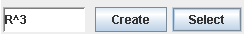
\includegraphics[scale=\largeshot]{moduleentry} \\
  \vspace{0.5cm}
  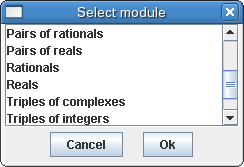
\includegraphics[scale=\largeshot]{modulelist}
  \caption{Module entry component (top), module list selection (bottom).}
\end{figure}


\subsubsection*{Form Entry (\incode{JSelectForm})}
\label{manual:subsubsec:formentry}

The entry of forms looks similar to the entry of modules, without the option to create a
new form. The \textscreen{Create} button is, however, available within the context of the
form builder tool.  The form is selected from the list. The form entry can be configured
to only allow specific types of forms. The types are shown at the top of the selection
window.
\begin{figure}[htb]
  \centering
  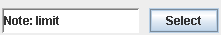
\includegraphics[scale=\largeshot]{formentry} \\
  \vspace{0.5cm}
  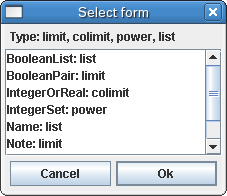
\includegraphics[scale=\largeshot]{formlist}
  \caption{Form entry component (top), form list selection (bottom).}
\end{figure}


\subsubsection*{Denotator Entry (\incode{JSelectDenotator})}
\label{manual:subsubsec:denoentry}

The denotator entry component is analogous to the form entry component. It can be
configured to only allow denotators with a specific form.
\begin{figure}[htb]
  \centering
  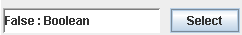
\includegraphics[scale=\largeshot]{denoentry} \\
  \vspace{0.5cm}
  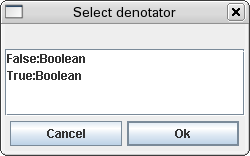
\includegraphics[scale=\largeshot]{denoselect}
  \caption{Denotator entry component (top), denotator list selection (bottom).}
\end{figure}


\subsubsection*{Module Element Entry (\incode{JModuleElementEntry})}
\label{manual:subsubsec:elemententry}

This component is shown whenever the user is required to specify a module element, i.e.,
numbers, vectors, strings, etc. It is always configured to accept elements from a
specified module. The use is straightforward, a more complicated case is shown in
\autoref{manual:fig:elemententry}, where the module in question is
$(\mathbb{Z}[X]\times\mathbb{R})^3$.
\begin{figure}[htb]
  \centering
  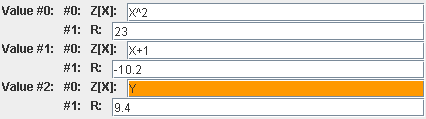
\includegraphics[scale=\largeshot]{elemententry} \\
  \caption{Module element entry for the module $(\mathbb{Z}[X]\times\mathbb{R})^3$.}
  \label{manual:fig:elemententry}
\end{figure}
The module of dimension $3$ is over the product ring $\mathbb{Z}[X]\times\mathbb{R}$,
where $\mathbb{Z}[X]$ is the polynomial ring with indeterminate $X$ and coefficients in
$\mathbb{Z}$. As can been seen, the first factor of the third component is incorrect,
since the polynomial indeterminate is not $Y$. This indicated by an orange background.


\subsubsection*{Module Morphism Entry (\incode{JMorphismEntry})}
\label{manual:subsubsec:modmorphentry}

Module morphisms can be built (button \textscreen{Create}), selected from a list of
predefined morphisms (button \textscreen{Select}), and prepared for editing (button
\textscreen{Edit}). Note that the dialog for editing may be different from the one
used for creating the morphism in the first place. The reason for this is that a morphism
of a specific type (for example affine) may be created using a variety of methods (matrix,
graphical) that can no longer be inferred for the edit operation (in this case, always
the matrix method will be used for editing). The \textscreen{Build} and \textscreen{Create}
actions invoke a module morphism builder dialog.
\begin{figure}[htb]
  \centering
  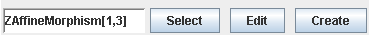
\includegraphics[scale=\largeshot]{mmorphismentry}
  \caption{Module morphism entry component.}
\end{figure}


\subsubsection*{Inputs/Outputs Sliders (\incode{JConnectorSliders})}
\label{manual:subsubsec:sliders}

Rubette properties may change the number of input and output connectors.  This component
provides a slider that can be configured to the minimum and maximum (at most 8) number of
connectors.
\begin{figure}[htb]
  \centering
  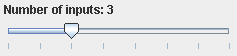
\includegraphics[scale=\largeshot]{slider}
  \caption{Slider for number of input connectors.}
\end{figure}

\subsubsection*{Path Selector (\incode{JFormTree})}
\label{manual:subsubsec:pathselect}

A denotator can be regarded as a tree, while its form specifies the structure of the
tree. It is sometimes necessary to pick a specific node from the form tree. This results in
a path from the root to this node. This path can later be used to perform operations on
this node in a denotator. The path selector (or form tree) is the corresponding user
interface component.
\begin{figure}[htb]
  \centering
  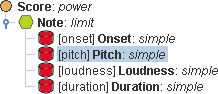
\includegraphics[scale=\largeshot]{pathselect}
  \caption{Path selector (or form tree), where the form \emph{Score} is expanded, and the
    path from the root \emph{Score} to the form \emph{Pitch} is selected.}
\end{figure}


\section{Core Rubettes}
\label{manual:sec:corerubettes}


\subsection{Rubette Description Schema}
\label{manual:subsec:schema}

To describe a rubette a common schema is used. The following layout shows all possible
components. Not all items have to be present. For example a rubette without view will not
include the \textit{View} item.

\begin{rubette}{Name}
  \group The group that the rubette belongs to. The rubettes in this section all belong to
  the group core, so it is not specified.
  \summary A short overview of the rubette.
  \inputs Enumeration and description of all input connectors.
  \outputs Enumeration and description of all output connectors.
  \description An exhaustive description of the rubette.
  \view An explanation of the view, if the rubette has one.
  \properties An explanation of the properties, if the rubette has any.
\end{rubette}

A rubette is implemented as a Java class, for example \incode{ExampleRubette}, the name is
then usually just ``\textbf{\textit{Example}}''.


\subsection{List of Core Rubettes}

The list is in alphabetical order. It may be possible that the list is incomplete with
respect to the latest version of \composer{} (available from \url{http://www.rubato.org}).

\begin{rubette}{AddressEval}
  \summary Evaluates a denotator at a specified address.

  \inputs \#1: The input denotator to be evaluated.

  \#2: When \emph{Evaluate at input denotator} is selected, this is the point at which is
  evaluated, it must be a denotator of type \Simple{} with the appropriate module.

  \outputs \#1: The evaluated denotator. In the case where several evaluations are
  requested (\emph{Evaluate at list of elements}), this is a set of evaluated denotators.

  \description This rubette performs address changes of denotators in general. There are
  several possibilities:

  \emph{a) Evaluate at null}: The address of the input denotator is changed to be the null
  module over the ring of the current address by evaluating the
  denotator at the zero element of its address.

  \emph{b) Evaluate at module element}: This is a slight generalization of \emph{Evaluate at null}.
  In this case the element used for evaluation is not the zero element, but an element specified
  in the properties.

  \emph{c) Evaluate at list of elements}: Similar to \emph{Evaluate at module element}, but
  with multiple evaluations, one for each element in a list specified in the
  properties. The result is no longer a denotator with the same form as the input form,
  but a form of type \List{} or \Power{} with the input form as coordinate form.
  
  \emph{d) Evaluate at input denotator}: Similar to \emph{Evaluate at module element}, but the
  module element is not specified in the properties but comes from input denotator \#2.

  \emph{e) Change address}: The most general alternative requires the specification of the address
  changing module morphism.

  \properties 
  \emph{Ad b)} The module element must be specified.

  \emph{Ad c)} A list of module elements must be specified (see \autoref{manual:fig:addresseval}).
  \begin{listfigure}%
    \centering
    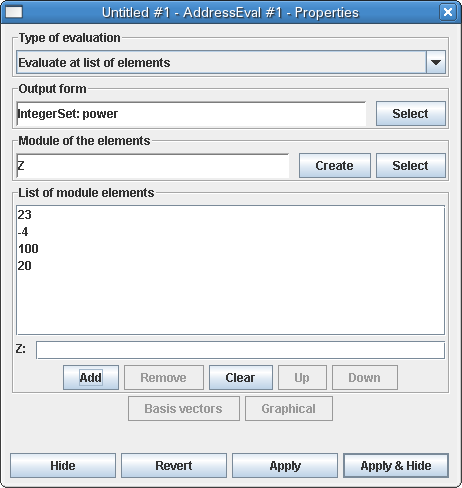
\includegraphics[width=\linewidth]{addresseval}
    \caption{The properties of the \emph{AddressEval} rubette, where \emph{Evaluate at list of elements} is
      selected.}
    \label{manual:fig:addresseval}
  \end{listfigure}%
  The list can be changed using the buttons at the bottom. The \textscreen{Basis vectors}
  button generates the list of canonical affine basis vectors of the module. In the case
  of $\mathbb{C}$ or $R^2$, where $R\in\{\mathbb{Z},\mathbb{Z}_n,\mathbb{Q},\mathbb{R}\}$,
  the button \textscreen{Graphical} opens a dialog, where the elements can be selected as
  points in the plane. Additionally, the output form must be selected from the forms of
  type \List{} or \Power{} with coordinate form equal to the form of the input denotator.

  \emph{Ad d)} The result form must be specified.

  \emph{Ad e)} The address changing module morphism must be specified.

  In the case of \emph{b)} and \emph{c)}, the address module must be specified.
\end{rubette}


\begin{rubette}{Boolean}
  \summary Evaluates a logical expression with the input denotators as variables.

  \inputs \#1--\#$n$: The variables (of form \emph{Boolean}) for the logical expression (default: $n=2$).

  \outputs \#1: The result (of form \emph{Boolean}) of the logical expression.

  \description A logical expression is evaluated, where the input denotators are
  variables. The syntax of logical expressions uses the parentheses \textscreen{(} and
  \textscreen{)}, the symbols \textscreen{\&} for logical conjunction, \textscreen{|} for
  disjunction, \textscreen{!} for negation, the constants \textscreen{T} and
  \textscreen{F}, the variables \textscreen{\#}$n$ for input denotators \#$(n+1)$, etc., and the
  usual precedence rules.

  \properties The number of arguments and the logical expression string must be set.
\end{rubette}


\begin{rubette}{Constructor}
  \summary Creates a denotator of the specified (non-\Simple) form.

  \inputs \#1--\#$n$: The coordinates of the result denotator. 

  \outputs \#1: The result denotator of the specified form.

  \description A denotator of the specified form is constructed using the coordinate
  denotators at the input connectors. The meaning of the input connectors changes with
  the type of the result denotator:

  \Power, \List: The input denotators form the elements of the result denotator. At
  most $8$ elements can be put it. Not all input connectors need to be actually
  connectors. For type \List{} the order is the left to right order of the connectors.

  \Limit: The input denotators are the coordinates of the \Limit{} denotator. Only
  the first $8$ factors can be specified, the excess coordinates are set to default
  denotators.

  \Colimit: The input denotator is the cofactor of the \Colimit{}
  denotator. The first non-null denotator will be the actual coordinate of the result
  denotator.

  \properties The form of the result denotator must be specified.
\end{rubette}


\begin{rubette}{Display}
  \summary Shows a textual representation of a denotator.

  \inputs \#1: The denotator to be shown.

  \description The input denotator is shown in a text window of the view. The
  representation can be either a simple human readable text or the complete XML text that
  is used for the file format. The \emph{Display} rubette is useful for debugging
  purposes.
  
  \view The main part is the text window. At the bottom is a switch that selects between
  simple and XML text.
\end{rubette}


\begin{rubette}{Latch}
  \summary Stores an input denotator and distributes it to one or more outputs.

  \inputs \#1: The input denotator.
  
  \outputs \#1--\#$n$: The output denotators \#$i$ are all the same.

  \description The denotator at the unique input connector is stored within the rubette
  and passed on to all of the output connectors. This may be useful for creating more
  branches from a single link.

 \properties The number of outputs can be set from $1$ to $8$.
\end{rubette}


\begin{rubette}{List}
  \summary Performs a list operation on the input denotators.

  \inputs
  \emph{(Concatenate)} \#1--\#$n$: The argument denotators of type \List{} (default $n=2$).

  \emph{(Concatenate All)} \#1: A list of denotators of type \List.

  \emph{(Append elements, Prepend elements)} \#1: A denotator of type \List.

  \#2--\#$n$: Denotators with form equal to the coordinate form of \#1 (default $n=2$).

  \emph{(Sort)} \#1: A denotator of type \List.
    
  \outputs \#1: The result of the list operation. The result form (of type \List) is
  taken from input denotator \#1, or in the case of \emph{Concatenate All}, the coordinate form
  of the form of input denotator \#1.

  \description The input denotators are the arguments to a list operation:

  \emph{Concatenate:} All input denotators are concatenated in the order of the inputs.

  \emph{Concatenate All:} The elements of the input denotator of type \List{} are
  concatenated in the order they occur in the input denotator.

  \emph{Append elements (Prepend elements):} The input denotator \#2--\#$n$ (where $n$ can
  be configured to be a value from 2 to 8), are appended (prepended) to the input
  denotator \#1.  The constraint is that these denotators have as form the coordinate form
  of the form of denotator \#1.

  \emph{Sort:} The result is the sorted input denotator \#1, according to the canonical
  order of denotators.

 \properties The list operation can be selected and the number of inputs for the operations 
 \emph{Concatenate}, \emph{Append (Prepend) elements} can be set.
\end{rubette}


\begin{rubette}{MacroInput}
  \summary Retrieves the inputs in a macro rubette.

  \outputs \#1--\#$n$: Each output connector \#$i$ will act as the input connector \#$i$ in the
  resulting macro rubette (default: $n=1$).

  \description This type of rubette only makes sense if it is placed in a network that is intended
  to be made into a macro rubette. It provides the external inputs to the macro rubette.

  \properties The number of output connectors can be specified, as well as a label for each output
  connector, which will show up later as a tooltip for the corresponding input connector on the
  macro rubette.
\end{rubette}


\begin{rubette}{MacroOutput}
  \summary Provides the outputs in a macro rubette.

  \inputs \#1--\#$n$: Each input connector \#$i$ will act as the output connector \#$i$ in the
  resulting macro rubette (default: $n=1$).

  \description This type of rubette only makes sense if it is placed in a network that is intended
  to be made into a macro rubette. It provides the external outputs from the macro rubette.

  \properties The number of input connectors can be specified, as well as a label for each input
  connector, which will show up later as a tooltip for the corresponding output connector on the
  macro rubette.
\end{rubette}


\begin{rubette}{ModuleMap}
  \summary Maps a module morphism onto a denotator.

  \inputs \#1: The input denotator.

  \outputs \#2: The mapped output denotator.

  \description Given a path from the root of a denotator to a node containing a denotator
  of type \Simple, a denotator is produced with the selected node or nodes replaced
  by the result of mapping a module morphism.

  \properties The input form, a path to a node of type \Simple, and a suitable module
  morphism must be selected.
\end{rubette}


\begin{rubette}{Mux}
  \summary Selects an input denotator according to the number given by input denotator \#1
  (also known as \emph{multiplexer}).

  \inputs \#1: A denotator of type \Simple{} with module $\mathbb{Z}$ containing a
  number.

  \#2--\#$n$: Input denotators, one of which is selected (default: $n=2$).

  \outputs \#1: The selected denotator.

  \description Input denotator \#1 must contain an integer $i$ between $2$ and $n$ (the
  configured number of inputs). The output is set to the input denotator \#$i$.

  \properties The number of input denotators can be set from $2$ to $8$.
\end{rubette}


\begin{rubette}{RealArith}
  \summary Evaluates an expression of real arithmetic with the input denotators as variables.

  \inputs \#1--\#$n$: The variables for the expression (default: $n=1$). The input
  denotators must be of type \Simple{} with module $\mathbb{R}$.

  \outputs \#1: The result of the arithmetical expression. In the case of a real result,
  the form of the result is taken to be the form of input denotator \#1. In the case of a
  Boolean result, the form is \emph{Boolean}.

  \description An expression of real arithmetic is evaluated, where the input denotators
  are variables. The syntax of expressions uses the parentheses \textscreen{(} and
  \textscreen{)}, real number constants and the binary operators \incode{+}, \incode{-},
  \incode{*}, \incode{/}, and \incode{\^{}}.  

  A ternary operator \textscreen{if}\ldots\textscreen{then}\ldots\textscreen{else} is also
  provided. The condition in this operator is a Boolean expression, with relation symbols
  \incode{<}, \incode{>}, \incode{<=}, \incode{>=}, \incode{=}, \incode{!=}, and Boolean
  operators \incode{\&}, \incode{|}, and \incode{!}, and constants \incode{T} and
  \incode{F}.

  Some common functions are also provided, \incode{sin}, \incode{cos}, \incode{tan},
  \incode{log}, \incode{exp}, \incode{abs}, \incode{sqrt}, \incode{max} and
  \incode{min}. The function arguments are placed within parentheses and separated by
  commas.
  
  The variables are \textscreen{\#}$n$ for input denotators \#$(n+1)$, etc..
  The common  precedence rules are used throughout.

  The result may be configured to be a Boolean. In that case the top level expression is 
  a Boolean instead of an arithmetical expression.

  \properties The number of arguments (input connectors) is specified. An option indicates whether
  the result is real or Boolean.
\end{rubette}


\begin{rubette}{Reform}
  \summary Casts the input denotator to a new form.

  \inputs \#1: The input denotator to cast from.

  \outputs \#1: The output denotator with the new form.

  \description The input denotator is cast into the configured form.

  \properties The output form must be specified.
\end{rubette}


\begin{rubette}{Register}
  \summary Registers a copy of the input denotator.

  \inputs \#1: The input denotator to register a copy of.

  \outputs \#1: The registered denotator.

  \description A \emph{copy} of the unique input denotator is registered with a specified
  name in the system repository.

  \properties The name can be specified.
\end{rubette}


\begin{rubette}{Scheme}
  \summary Executes Scheme code on the input denotators.

  \inputs \#1--\#$n$: The input denotators, which can be accessed using the \incode{get-input}
  Scheme function.

  \outputs \#1--\#$n$: The output denotators, which can be written using the \incode{set-output}
  Scheme function.

  \description The specified Scheme code is executed. For example the expression
  \incode{(set-output 0 (get-input 0))}, sets the first output denotator to the first
  input denotator. The code runs in an environment on top of the global environment containing
  the standard Scheme bindings. The local environment is empty at the begin of each run. See
  also~\autoref{manual:sec:scheme}.

  \properties The number of input and output connectors, and the Scheme code to execute
  are specified.
\end{rubette}


\begin{rubette}{Select2D}
  \summary Projects a list or set of denotators to one or more planes, and returns a
  selection of them specified by polygons in the planes.

  \inputs \#1: Input denotator of type \List{} or \Power{} with specified coordinate form.

  \outputs \#1: Output denotator of the same form as input \#1, but containing only the
  selected elements.

  \description The elements of the input denotator are projected to one or more planes. On
  each projection, one or more polygonal selections can be drawn. The selected elements
  for each plane are the elements whose projected coordinates lie in one of the polygons.
  The final selection is the intersection of the selections of all planes.

  \properties The input coordinate form must be specified first. Then a selection tab can
  be created, and the projected coordinates for the $x$- and $y$-axes are specified using
  path selectors. Selection tabs can be added and removed.

  Polygonal selections can be created (first toolbar button), selected for editing (second
  button), vertexes added (third button), removed (fourth button) and moved (fifth button).
  Other operations are: information about a point and zooming (see \autoref{manual:fig:select2d}).
  \begin{listfigure}%
    \centering
    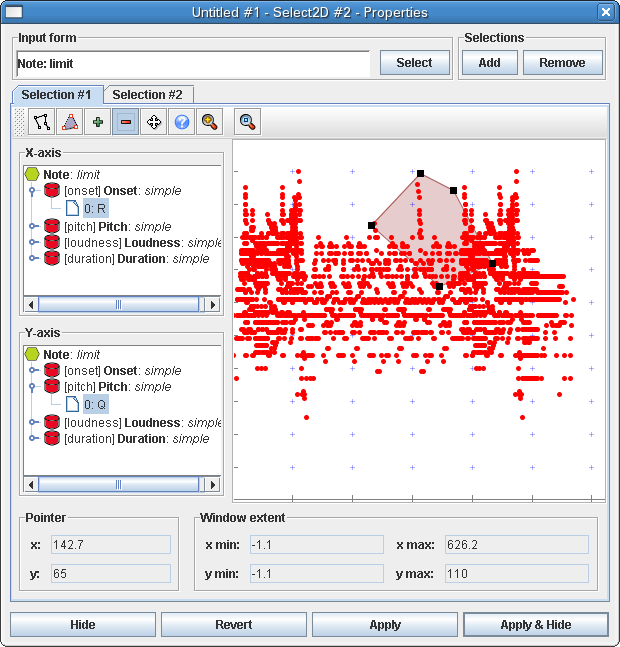
\includegraphics[width=\linewidth]{select2d}
    \caption{The properties of the \emph{Select2D} rubette. Here the first of two
      selection tabs is visible. The coordinate form is \emph{Note}, the projection on the
      $x$-axis is the $\mathbb{R}$ ring of its \emph{Onset} coordinate, the projection on the
      $y$-axis is the $\mathbb{Q}$ ring of its \emph{Pitch} coordinate. A single polygonal
      selection has been drawn. Also visible are the current position of the pointer and
      the extents of the window.}
    \label{manual:fig:select2d}
  \end{listfigure}%
\end{rubette}


\begin{rubette}{SelectForm}
  \summary Retrieves all denotators with a specified form contained somewhere in the input
  denotator tree.

  \inputs \#1: The input denotator.

  \outputs \#1: A denotator of type \List{} or \Power{} containing the collection
  of denotators retrieved from the input denotator.

  \description The input denotator tree is traversed and all denotators of the specified
  form are collected. The output denotator is a list or set containing the resulting
  collection as elements.  It is, however, not the form itself that is specified, but the
  output form, which can be of type \Power{} or of type \List{}. The query form is then
  its coordinate form.

  \properties The output form of type \List{} or \Power{} must be specified.
\end{rubette}


\begin{rubette}{Set}
  \summary Performs a set operation on the input denotators.

  \inputs
  \emph{(Union, Intersection, Difference, Symmetric Difference)} \#1--\#$n$: The argument denotators
  of type \Power{} (default: $n=2$).

  \emph{(Add Element)} \#1: A denotator of type \Power.

  \#2--\#$n$: Denotators with form equal to the coordinate form of \#1 (default $n=2$)

  \emph{(Big Union (Intersection))} \#1: A set or list of denotators of type \Power.

  \outputs \#1: The result of the set operation.  The result form (of type \Power) is
  taken from input denotator \#1, or in the case of \emph{Big Union (Intersection)}, the
  coordinate form of the form input denotator \#1.

  \description The input denotators are the arguments to a set operation: 

  \emph{Union, Intersection, Difference, Symmetric Difference:} The specified operation is
  performed on the input denotators.

  \emph{Add Element:} Input denotators \#2--\#$n$ are added to the elements of input
  denotator \#1.

  \emph{Big Union (Intersection):} The result is the union (intersection) of all
  denotators, elements of the input denotator.

  \properties The set operation is selected and the number of input denotators where
  appropriate.
\end{rubette}


\begin{rubette}{Simple}
  \summary Produces a denotator of type \Simple.

  \outputs \#1: A denotator of type \Simple.

  \description A denotator of type \Simple{} is stored and put to the output
  connector.

  \properties A form of type \Simple{} is selected. An option specifies if the
  denotator should be null-, or non-null-addressed. If null-addressed, the module element,
  otherwise a module morphism, must be entered (see \autoref{manual:fig:simplerubette}).
  \begin{listfigure}%
    \centering
    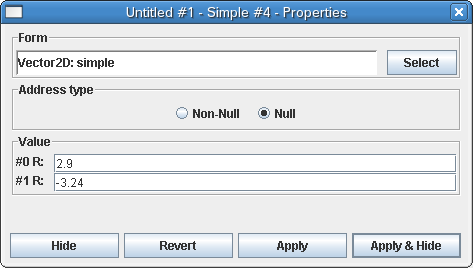
\includegraphics[width=\linewidth]{simplerubette}
    \caption{The properties of the \emph{Simple} rubette. The module in this case is
       the Euclidean plane $\mathbb{R}^2$.}
    \label{manual:fig:simplerubette}
  \end{listfigure}%
\end{rubette}


\begin{rubette}{Source}
  \summary Produces a registered denotator at its output.

  \outputs \#1: Specified output denotator.

  \description A denotator is specified and delivered to the only output connector. The
  denotator is selected from all registered denotators. Therefore only non-anonymous
  denotators can be specified.

  \properties The denotator is specified using a denotator entry component. Additionally
  it can be indicated whether during execution the named denotator is always retrieved
  anew from the repository (\textscreen{Self-refreshable} is selected). This is useful if
  a new denotator is registered under that name.
\end{rubette}


\begin{rubette}{Split}
  \summary An input denotator of type \Limit{} is split into its factors.

  \inputs \#1: A denotator of type \Limit{}.

  \outputs \#1--\#$n$: The factors of the \Limit{} denotator that have been selected in the
  properties.

  \description The input denotator of type \Limit{} is split into its factors, which
  are produced on the output connectors. In the properties, the factors to output are
  selected from the list of all factors.
\end{rubette}


\begin{rubette}{Stat}
  \summary Performs a statistical operation.

  \inputs \#1: Input denotator containing the values to process.

  \outputs \#1: The result (denotator of type \Simple{} with a specified form) of the
  statistical operation.

  \description The set of all denotators with a specified form (of type \Simple) is
  extracted from the input denotator, and a statistical operation is performed on this
  set. Available operations are \emph{Minimum}, \emph{Maximum}, \emph{Mean},
  \emph{Variance}, \emph{Sum} and \emph{Product}. Not all modules allow every operation.

  \properties The form (of type \Simple{} to extract, which is also the form of the
  output denotator) can be specified as well as the type of operation.
\end{rubette}


\section{Built-in Non-Core Rubettes}
\label{manual:sec:noncorerubettes}

\composer{} contains several non-core rubettes, mostly related to music. These rubettes do
not belong to the \emph{Core} group since they are more application specific.

\begin{rubette}{MidiFileIn}
  \group Score

  \summary Reads a MIDI file and converts it to a denotator of form \emph{Score}.

  \outputs \#1: A denotator of form \emph{Score}.

  \description The specified MIDI file is read and converted to a denotator of form
  \emph{Score}. Only the attributes onset, pitch, duration, and loudness of the MIDI note
  events are considered.
  
  \properties The MIDI file to load is selected using the usual open file dialog.
\end{rubette}

\begin{rubette}{MidiFileOut}
  \group Score

  \summary Converts a denotator of form \emph{Score} to MIDI and writes it to a file.

  \inputs \#1: A denotator of form \emph{Score},

  \description The input denotator of form \emph{Score} is converted and written to the
  specified MIDI file. Since the \emph{MidiFileIn} rubette discards information, a MIDI
  file read in using \emph{MidiFileIn} will not be the same when written back using
  \emph{MidiFileOut}.

  \properties The MIDI file to write to is selected using the usual open file dialog.
\end{rubette}

\begin{rubette}{ScorePlay}
  \group Score

  \summary Displays and plays a denotator of form \emph{Score}.

  \inputs \#1: A denotator of form \emph{Score}.

  \description The input denotator of form \emph{Score} is displayed in the \emph{view}
  window as a piano roll and can be played using common media player controls.

  \view The greatest part of the view (\autoref{manual:fig:scoreplay}) is occupied by the score
  in piano roll representation, familiar from sequencer software. Onset, duration and
  pitch are obviously coded as bars, loudness by varying color saturation, and the voice of
  the note by different color hues (red, blue, etc.).
  
  \begin{listfigure}%
    \centering
    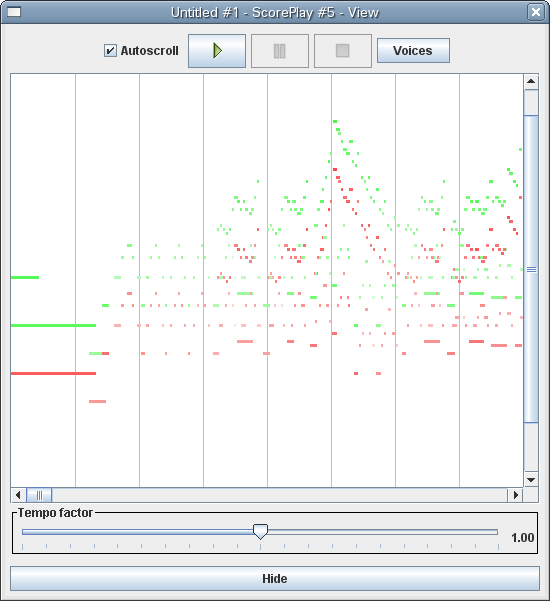
\includegraphics[scale=0.5]{scoreplay}
    \caption{The view of the \emph{ScorePlay} rubette.}
    \label{manual:fig:scoreplay}
  \end{listfigure}%

  The top line of buttons trigger the actions play, pause and stop, from left to right.
  During playback a moving vertical line will show the current position in the piano roll
  window. The window is scrolled with the vertical line, unless the
  \textscreen{Autoscroll} check box is unchecked.

  The piano roll representation can be zoomed in and out horizontally by pressing the
  \textkey{Page Up} (zooming in by a factor of 2, up to 3 steps) and \textkey{Page Down}
  (zooming out by a factor of 2, up to 3 steps) keys.

  By clicking within the piano roll, the playing position is set to that point. If playing
  is stopped, it will be started.

  The \textscreen{Voices} button opens a dialog that allows the assignment of General
  MIDI instruments to voices (\autoref{manual:fig:voices}). From the top combo box the voice to
  change can be selected from all voices actually present in the score.

  \begin{listfigure}
    \centering
    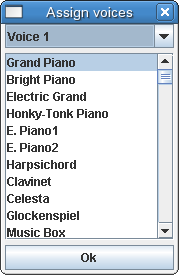
\includegraphics[scale=0.7]{voices}
    \caption{Assignment of instruments to voices (\emph{ScorePlay} rubette).}
    \label{manual:fig:voices}
  \end{listfigure}

  At the bottom a slider allows the adjustment of the playback tempo factor.
\end{rubette}


\section{Writing Rubettes}
\label{manual:sec:writingrubettes}

\composer{} essentially depends on the availability of useful rubettes. The previous
sections described a core set that is always present. For specific applications,
third-party rubettes designed as plug-ins are expected to enrich the environment.  In this
section, a short overview and tutorial will introduce the potential developer to the
mechanisms of rubette design.

Currently the only supported language is Java. This introduction will therefore reference
Java packages, interfaces and classes as they are implemented in the \rubato{} framework.


\subsection{Using the \textsc{Rubato} Framework}
\label{manual:subsec:usingframework}

There is no place in this manual for a complete exposition of the \rubato{} class
hierarchy. It is enough to give pointers to the important packages. For the details, the
reader should peruse the extensive Javadoc generated from sources itself, and therefore
always up-to-date.
\begin{itemize}
\item The core framework dwells under the package \incode{org.rubato.math}. This contains
  the complete implementation of the mathematical foundation of modules, forms and
  denotators.
\item Modules and elements of modules are contained in the package
  \incode{org.rubato.math.module}, morphisms between modules in the package
  \incode{org.rubato.math.module.morphism}. They make use of several classes such as for
  complex numbers, modular arithmetic, string rings and matrixes from the packages
  \incode{org.rubato.math.arith} and \incode{org.rubato.math.matrix}.
\item The package \incode{org.rubato.math.yoneda} contains the classes for forms and
  denotators.
\item The packages starting from \incode{org.rubato.logeo} collect general operations and
  algorithms on denotators, such as set operations for power denotators and list
  operations for list denotators. There are also tools for the simplified construction of
  denotators and forms.
\item The developer of rubettes also needs the package \incode{org.rubato.base}, which
  contains the \incode{Rubette} Java interface, the package \incode{org.rubato.xml} for
  reading and writing XML representations, as well as the packages
  \incode{org.rubato.composer.dialog} containing dialogs for entering the various types of
  objects, and \incode{org.rubato.composer.components} for special widgets useful for the
  implementation of rubette properties and view dialogs.
\item General utilities can be found in the package \incode{org.rubato.util}.
\end{itemize}

One remark that applies to the development in \rubato{} in general: Before a newly created
form can be used to create a denotator, it must be \emph{registered}. This ensures that
names are bound to forms in a unique way. This constraint does not apply to denotators.
Since this rule is so important, here is a code example to show how to do it:

\begin{java}
  import org.rubato.base.Repository;
  import org.rubato.logeo.FormFactory;
  $\cdots$
  Repository rep = Repository.systemRepository();
  Form f = FormFactory.makeZModuleForm("Integer");
  f = rep.register(f);
  if (f == null) {
    $\cdots$
  }
  $\cdots$  
\end{java}
The method \incode{register} returns \incode{null} in the case that the registration has
failed (which may happen when a form of that name has already been registered, for
example), thus the return value should always be checked.


\subsection{Rubette Interface}
\label{manual:subsec:rubetteinterface}

The Java interface that every rubette must implement is shown in
\autoref{manual:sec:rubjavainterface} on page~\pageref{manual:sec:rubjavainterface}. Before we embark
on the description of the methods in details, it is important to note that not every
method is intended to be used by the implementor of rubettes, nor is it even necessary to
implement all methods. In fact, in almost all cases, a rubette will inherit from the
abstract class \incode{AbstractRubette}, which provides default implementations for some
of the methods. The methods that are implemented in \incode{AbstractRubette} and are not
generally reimplemented in a specific rubette are marked with a bullet~($\bullet$). Those
that are given default implementations, but are usually overridden in the implementing
rubette class, are marked with a circle~($\circ$). Finally, those methods, that
\emph{must} be implemented are left unmarked.

A note about constructors: A rubette \emph{must} provide a default constructor (i.e., a
constructor with no arguments), since this is called when \composer{} instantiates the
prototype of the rubette. The default constructor can be overridden, for example to set
default values for the rubette parameters. Of course, other constructors can provided in
addition to the default constructor, see for example the code for \incode{fromXML} below.
\begin{basedescript}{%
    \labelsep=0em%
    \desclabelwidth{2em}%
    \desclabelstyle{\nextlinelabel}%
    \renewcommand{\makelabel}[1]{\incode{#1}}%
}
\item[void init()] This method is called whenever the rubette prototype is created. This
  is the place where global structures and variables can be created and initialized. By
  default, this method does nothing.

\item[void run(RunInfo \v{runInfo})] This method embodies the computational core of the
  rubette. Typically it starts by retrieving the inputs using \textscreen{getInput}, then
  it checks the inputs for correct form (inputs may be \textscreen{null}), and terminates
  by setting the results using \textscreen{setOutput}. The argument of type
  \textscreen{RunInfo} contains information about the current execution. The rubette
  should check \textscreen{runInfo.stopped()} periodically during long calculations. If
  this method return \textscreen{true}, \textscreen{run} should abort gracefully and
  return.

\item[Rubette newInstance()] Whenever a new instance of this rubette is created by
  \composer{}, this method is called on a prototype object. It must return a freshly and
  fully initialized object of this rubette. It is a kind of \emph{virtual constructor} and
  must not depend on global state. By default this method calls the default constructor of
  the rubette constructor.

\item[Rubette duplicate()] This method is called whenever the duplicate operation is
  invoked on a rubette in the GUI. It should return a copy of the rubette instance, which
  inherits as many attributes as possible. The default implementation is equivalent to
  \incode{newInstance}.

\item[void toXML(XMLWriter \v{writer})] Every rubette instance must be saveable to
  and loadable from a stream. The native format is XML and this method is responsible for writing
  a representation of the rubette instance. It is called by \composer{} and is surrounded
  by an XML tag \incode{Rubette} that already identifies the type of rubette. The body of
  this method is therefore responsible only for the settings specific to this rubette.  It
  can make use of all the utility methods defined by the \incode{XMLWriter} class from the
  package \incode{org.rubato.xml}. As an example, consider a rubette whose configuration
  only consists of an integer variable \incode{a} and a string variable \incode{s}:
\begin{quote}\begin{java}
public void toXML(XMLWriter writer) {
  writer.empty("A", "value", a);
  writer.empty("S", "value", s);
}
\end{java}\end{quote}
  If \incode{a}~$=5$ and \incode{s}~$=$~\incode{"Text"}, this results in the XML code:
\begin{quote}\begin{java}
<A value="5"/>
<S value="Text"/>
\end{java}\end{quote}
  Here the \incode{empty} method is used. Consult the Javadoc for the variety of different
  methods provided by \incode{XMLWriter}.

\item[Rubette fromXML(XMLReader \v{reader}, Element \v{element})] To parse the XML
  representation of a rubette of this type, this method, which is the inverse of
  \incode{toXML}, is called. The argument \incode{\v{element}} contains the list of
  XML elements written by \incode{toXML}. Taking up the previous example, the code
  that retrieves \incode{a} and \incode{s} would be:
\begin{quote}\begin{java}
Rubette fromXML(XMLReader reader, Element element) {
    // get element <A>, head of the list
    Element child = reader.getChild(element, "A");
    if (child == null) {
        // there is no element <A>
        return null;
    }
    // get value of element <A>, use default 0
    int a = reader.getIntAttribute(child, "value", 0);
    // get element <S>, next in list
    child = reader.getNextSibling(child, "S");
    if (child == null) {
        // there is no element <S>
        return null;
    }
    // get value of element <S>
    String s = reader.getStringAttribute(child, "value");
    ExampleRubette r = new ExampleRubette(a, s);
    return r;
}
\end{java}\end{quote}
  The class \incode{XMLReader} from package \incode{org.rubato.xml} provides many
  methods for parsing elements besides the ones used here.
  
  This method must return a new instance initialized according to the settings retrieved
  from XML. If there is an error, the return value must be \incode{null}. Error messages
  can be set using \incode{XMLReader.setError}, which works similarly to the
  \incode{addError} method described below.

\item[String getGroup()] Returns the group that this rubette belongs to. Core rubettes
  belong to the group \incode{``Core''}. An independent rubette should not belong to
  \incode{``Core''}. The return value can otherwise be any string whatever. The default
  group inherited from \incode{AbstractRubette} is \incode{``Other''}.

\item[ImageIcon getIcon()] Returns the icon that is displayed in the graphical
  representation of the rubette (see \autoref{manual:fig:rubette}).  This must be a fixed
  value, and not vary during the rubette's lifetime. The default return value is
  \incode{null}, which is equivalent to a blank icon.

\item[boolean hasProperties()] Must return \incode{true} if this rubette has a properties
  dialog. If \incode{true} the methods \incode{getProperties}, \incode{applyProperties}
  and \incode{revertProperties} must also be implemented.  The default value is
  \incode{false}.

\item[JComponent getProperties()] If \incode{hasProperties} returns \incode{true}, this
  must return a \incode{JComponent}, for example a \incode{JPanel} containing various
  user interface elements, buttons, sliders, etc. This component is placed by \composer{}
  in a window as shown in \autoref{manual:fig:proptemplate}.
  \begin{figure}[htb]%
    \centering
    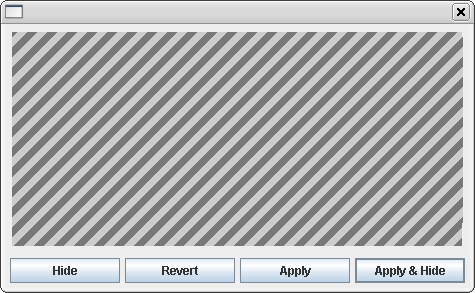
\includegraphics[scale=\largeshot]{proptemplate}
    \caption{Properties window container.}
    \label{manual:fig:proptemplate}
  \end{figure}%
  Four buttons are added: \textscreen{Hide} removes the window from view,
  \textscreen{Revert} calls the rubette's \incode{revertProperties} method,
  \textscreen{Apply} calls the rubette's \incode{applyProperties} method
  and \textscreen{Apply \& Hide} is a combination of both operations.

\item[boolean applyProperties()] This method is linked to the button \textscreen{Apply} in
  the properties dialog. It should make the changes that the user made in the properties
  dialog permanent.

\item[void revertProperties()] This method is linked to the button \textscreen{Revert} in
  the properties dialog. It should replace the values in the properties dialog by the
  current settings of the rubette.

  The last two methods imply that changes in the properties dialog must not take effect
  immediately, but only after the user presses the \textscreen{Apply} button.

\item[boolean hasView()] Must return \incode{true} if this rubette has a view.  If
  \incode{true}, the methods \incode{getView} and \incode{updateView} must also be
  implemented.  The default value is \incode{false}.

\item[JComponent getView()] If \incode{hasView} returns \incode{true}, this must return a
  \incode{JComponent}, for example a \incode{JPanel}. This component may be contain
  whatever is necessary to perform a multimedia rendering of the rubette's
  state. Similarly to the \incode{getProperties} method, the component is inserted by
  \composer{} in a window as shown in \autoref{manual:fig:viewtemplate}.
  \begin{figure}[htb]%
    \centering
    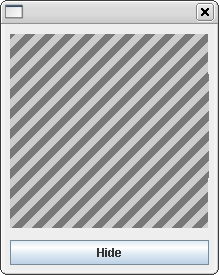
\includegraphics[scale=\largeshot]{viewtemplate}
    \caption{View window container.}
    \label{manual:fig:viewtemplate}
  \end{figure}%
  The only button, \textscreen{Hide}, causes the window to disappear. It can be shown
  again by clicking \textscreen{View} on the rubette.
  
\item[void updateView()] During the execution of a network, the state of the rubette may
  change, thus causing a change in its view. \composer{} calls \incode{updateView} to
  notify the rubette that it should update its view.

\item[boolean hasInfo()] Must return \incode{true} if this rubette has an information
  text. If \incode{true}, the method \incode{getInfo} must also be implemented.  The value
  must not vary during the rubette's lifetime. The default value is \incode{false}.

\item[String getInfo()] Returns the string for the information displayed on the graphical
  representation of the rubette (see \autoref{manual:fig:rubette}). This string must be short and
  must not contain line breaks. The value can vary during the rubette's lifetime.  The
  default value is \incode{null}.

\item[String getShortDescription()] Returns a short description of the rubette. This
  string is shown as a tooltip when the mouse pointer hovers over the rubette. The string
  must be short and must not end with a period for consistency. The default value is
  \incode{null}, which means no tooltip at all.

\item[String getLongDescription()] Returns a long description of the rubette. This string
  is displayed in the description area of the rubette panel when the rubette is selected.
  This string can be of arbitrary length and must end with a period for consistency. The
  default value is \incode{null}.

\item[String getInTip(int \v{i})] When the mouse pointer hovers over an input or output
  connector, a tooltip describing the connector can be displayed. This method should
  return a string for the tooltip of input connector number \incode{\v{i}}, where
  $0\leq\incode{\v{i}}<\incode{getInCount()}$.

\item[String getOutTip(int \v{i})] Analogous to \incode{getInTip}, this should return a
  string for the tooltip output connector number \incode{\v{i}}, where
  $0\leq\incode{\v{i}}<\incode{getOutCount()}$.

\item[void setInCount(int \v{n})] The number of input connectors is set using this method
  in the constructor of the rubette. The number can be changed during the lifetime of the
  rubette by adding such an option to the properties dialog. However if the number is
  reduced, those links that have been connected to those connectors that will not exist
  anymore will be removed.

\item[int getInCount()] Returns the current number of input connectors. There is not much
  sense in overriding the default implementation.

\item[Denotator getInput(int \v{i})] Returns the denotator at input connector number $i$,
  where $0\leq i< \incode{getInCount()}$. This method is normally called for each of the
  input connectors at the beginning of the \incode{run} method.

\item[void setOutCount(int \v{n})] The number of output connectors is set using this
  method in the constructor of the rubette. The number can be changed during the lifetime
  of the rubette by adding such an option to the properties dialog.  However if the number
  is reduced, those links that have been connected to those connectors that will not exist
  anymore will be removed.

\item[int getOutCount()] Returns the current number of output connectors. There is not much
  sense in overriding the default implementation.

\item[void setOutput(int \v{i}, Denotator \v{d})] Sets the result denotator at output connector
  number $i$, where $0\leq i< \incode{getOutCount()}$. This method is normally called for
  each of the output connectors at the end of the \incode{run} method.

\item[void addError(String \v{msg}, Object ... \v{objects})] If an error occurs during the
  calculation performed by the \incode{run} method, this method should be used to publish
  the error. It can, of course, be called multiple times, whenever it makes sense to
  continue after an error has occurred. The error message is specified using the argument
  \incode{\v{msg}}. This string can contain template variables of the form \incode{\%}$n$,
  where $n$ is a digit from $0$ to $9$. These variables are replaced by the arguments from
  \incode{\v{objects}} in this order. For convenience, the variable names \incode{\%\%}$n$
  may be used, in this case the corresponding argument is surrounded by double quotes
  (\incode{"}) in the resulting string.
  Thus \incode{addError("Input \%0 is \%1 in \%\%2", 2, "null", "ExampleRubette")} will
  generate the string \incode{"Input 2 is null in $\backslash$"ExampleRubette$\backslash$""}.

\item[%
  \begin{minipage}{\linewidth}%
    Denotator getOutput(int \v{i}) \\
    List<String> getErrors() \\
    void clearErrors() \\
    boolean hasErrors() \\
    void setModel(RubetteModel \v{model}) \\
    RubetteModel getModel() \\
  \end{minipage}]%
  These five methods are used internally by \composer{} and are of no use to the rubette
  implementor. They are declared \incode{final} and can therefore not be overridden in a
  subclass of \incode{AbstractRubette}.
\end{basedescript}


\section{Rubette Example}
\label{manual:sec:rubetteexample}

The example for writing a rubette presented in this section is based on the \emph{Latch}
rubette. It is simple enough to only use the basic functionality of the \rubato{}
framework, but incorporates most features of a rubette implementation.


\subsection{Specification}

The \emph{Latch} rubette has one input connector and a configurable number of output
connectors (from 1 to 8, the default should be 1). On execution, the rubette will forward
the input denotator to each of the output connectors.

This specification makes clear that the rubette will feature a properties dialog to set
the number of output connectors, and no view.


\subsection{The LatchRubette class}

The class \incode{LatchRubette} resides in an arbitrary package, say
\incode{rubatoexample.LatchRubette}:
%
\begin{quote}\begin{java}
package rubatoexample.LatchRubette;

// here come the necessary import statements

public class LatchRubette extends AbstractRubette {
$\ldots$
}
\end{java}\end{quote}
%

The methods that must be implemented are presented in the following.

The default constructor is the right place to set the number of input connectors and the
default number of output connectors. The \incode{init} method does not need to be
implemented, since the rubette does not use any additional data structures that must be
initialized beforehand, for example forms or denotators. The only configurable attribute
is the number of output connectors and this will be transferred to the copy in the
\incode{duplicate} method. Instead of setting the attribute after creating a rubette
instance using the default constructor, an additional constructor could have been created
which takes as argument the number of output connectors.
%
\begin{quote}\begin{njava}
public LatchRubette() {
    setInCount(1);
    setOutCount(1);
}

public Rubette duplicate() {
    LatchRubette rubette = new LatchRubette();
    rubette.setOutCount(getInCount());
    return rubette;
}
\end{njava}\end{quote}
\lstset{firstnumber=last}
Now for the informational methods. The rubette should be called ``\incode{Latch}'' and
belong to the group ``\incode{Examples}''.
%
\makeatletter\advance\c@lstnumber1\makeatother
\begin{quote}\begin{njava}
public String getName() {
    return "Latch";
}

public String getGroup() {
    return "Examples";
}
\end{njava}\end{quote}
%
The short description explains the function of the rubette in the most concise way,
whereas the long description gives an expanded version thereof. In more complex rubettes,
the long description usually gives a few hints for the usage of the rubette. The methods
specifying the tooltips of the connectors do not contain any special information in the
case of this simple rubette. If the connectors played different roles, these methods would
give a hint to their meaning.  Here, the output connector tooltip depends on the actual
position of the output connector.
%
\makeatletter\advance\c@lstnumber1\makeatother
\begin{quote}\begin{njava}
public String getShortDescription() {
    return "Stores an input denotator";
}

public String getLongDescription() {
    return "The Latch Rubette stores its input denotator"+
           " and provides it on its outputs the number of"+
           " which can be configured.";
}

public String getInTip(int i) {
    return "Input denotator";
}

public String getOutTip(int i) {
    return "Output denotator #"+i;
}
\end{njava}\end{quote}
%
For the icon, it is necessary to load an image. If this image (for example a PNG file such
as \incode{latchicon.png}) is stored in the same directory as the package of the rubette,
the method \incode{loadIcon} from the utility class \incode{Icons} can be used. It takes
as first argument the rubette class, and as second argument the file name. The icon is
loaded statically and stored in a class variable.  It should be a pixmap of size
$16\times16$ pixels.
%
\makeatletter\advance\c@lstnumber1\makeatother
\begin{quote}\begin{njava}
public ImageIcon getIcon() {
    return icon;
}

private final static ImageIcon icon;

static {
    icon = Icons.loadIcon(LatchRubette.class, "latchicon.png");
}
\end{njava}\end{quote}

The most important method is the core method \incode{run}. In this case it is very simple:
it puts the sole input denotator to each output denotator.  For illustration purposes the
code is slightly extended to make use of the \incode{runInfo} parameter. The \incode{run}
method returns if it has been detected that execution has been stopped
(line~\ref{manual:ex:stopped}).
%
\makeatletter\advance\c@lstnumber1\makeatother
\begin{quote}\begin{njava}
public void run(RunInfo runInfo) {
    Denotator d = getInput(0);
    for (int i = 0; i < getOutCount(); i++) {
        if (runInfo.stopped()) {$\label{manual:ex:stopped}$
            return;
        }
        setOutput(i, d);
    }
}
\end{njava}\end{quote}

Since there is no view, the corresponding methods can be left untouched. There is,
however, a properties dialog for setting the number of outputs. The method
\incode{hasProperties} must therefore return \incode{true} and the three other methods
related to the properties dialog must be implemented.
%
\makeatletter\advance\c@lstnumber1\makeatother
\begin{quote}\begin{njava}
public boolean hasProperties() {
   return true;
}

public JComponent getProperties() {
    if (properties == null) {
        properties = new JPanel();$\label{manual:ex:jpanel}$
        properties.setLayout(new BorderLayout());

        outSlider = new JConnectorSliders(false, true);$\label{manual:ex:outslider}$
        outSlider.setOutLimits(1, 8);$\label{manual:ex:outlimits}$
        outSlider.setOutValue(getOutCount());$\label{manual:ex:outcount}$
        properties.add(outSlider, BorderLayout.CENTER);$\label{manual:ex:border}$
    }
    return properties;
}

public boolean applyProperties() {
    setOutCount(outSlider.getOutValue());$\label{manual:ex:setout}$
    return true;
}

public void revertProperties() {
    outSlider.setInValue(getOutCount());$\label{manual:ex:revert}$
}

private JPanel properties = null;
private JConnectorSliders outSlider = null;
\end{njava}\end{quote}
%
The properties dialog is constructed once for each rubette and saved in a field
\incode{properties}. It features a \incode{JConnectorSliders} component
(line~\ref{manual:ex:outslider}) that is configured to provide an output connector slider
(the second argument is \incode{true}) and no input connector slider (the first argument
is \incode{false}), since the number of input connectors is fixed to one.  Additionally
the limits are set to be from $1$ to $8$ (line~\ref{manual:ex:outlimits}) and the current
value is set to the current number of output connectors (line~\ref{manual:ex:outcount}).
The component is then placed in a \incode{JPanel} (line~\ref{manual:ex:jpanel}) using a
\incode{BorderLayout} (line~\ref{manual:ex:border}).  The configuration is applied by
setting the current number of output connectors from the current value of the slider
(line~\ref{manual:ex:setout}).  To revert, the slider value is set from the current number
of output connectors (line~\ref{manual:ex:revert}).

The last step is the implementation of the methods for writing to and reading from XML.
%
\makeatletter\advance\c@lstnumber1\makeatother
\begin{quote}\begin{njava}
private final static String OUTPUTS = "Outputs";$\label{manual:ex:outputconst}$
private final static String NUMBER_ATTR = "number";$\label{manual:ex:outputattr}$
        
public void toXML(XMLWriter writer) {
    writer.empty(OUTPUTS, NUMBER_ATTR, getOutCount());$\label{manual:ex:xmlwrite}$
}
    
public Rubette fromXML(XMLReader reader, Element element) {
    Element child = reader.getChild(element, OUTPUTS);$\label{manual:ex:getchild}$
    if (child != null) {
        int n = reader.getIntAttribute(child, NUMBER_ATTR, 1, 8, 1);$\label{manual:ex:getnumber}$
        LatchRubette rubette = new LatchRubette();
        rubette.setOutCount(n);
        return rubette;
    }
    else {
        return null;
    }
}    
\end{njava}\end{quote}
%
The only setting that must be saved is the number of output connectors $n$. A constant
string for the tag is defined, as well as the attribute in this tag for the number $n$
(lines~\ref{manual:ex:outputconst}--\ref{manual:ex:outputattr}).

To write XML, the method \incode{empty} from the writer instance is used
(line~\ref{manual:ex:xmlwrite}). If $n=3$ for example, this results in the string:
\begin{quote}
\begin{verbatim}
    <Outputs number="3"/>
\end{verbatim}
\end{quote}
Reading from XML is a little more complicated, since error checking must be performed. The
method starts by retrieving the first child of the \incode{Rubette} element, which is
passed as argument to the \incode{fromXML} method. This child should contain an element
with the \incode{Outputs} tag.  If it is \incode{null}, parsing has failed and
\incode{null} is returned to mark this event as an error.  Otherwise the value of the
attribute \incode{number} in element \incode{Outputs} is retrieved using the method
\incode{getIntAttribute} from the reader object. The two first argument numbers indicate
the expected range of the value and the method will clamp the received value to this
range. If parsing fails, the third argument number is returned as the default value.  If
everything has been parsed correctly, an instance of the rubette is created and the number
of output connectors is configured on this instance.

The complete, fully functional source code is contained in \autoref{manual:app:example}.


\subsection{Making a Plug-In}
\label{manual:subsec:plugin}

One possibility to make the rubette available to \composer{} consists in compiling it into
the distribution. To do this, the Java file \incode{org.rubato.composer.BuiltinRubettes}
has to be adapted by extending the arrays \incode{classes} of strings by the fully
qualified name of the rubette class. To avoid this, the plug-in mechanism should be used.
The rubette, including its supporting classes, but not classes from the standard \rubato{}
framework, is put into a JAR archive. In order that \rubato{} can find the rubette, the
manifest of the JAR file needs to specify the name of the rubette class. In the case of
the Latch rubette a file named \textscreen{manifest} with the following content has to be
created:
\begin{quote}
\begin{verbatim}
Plugin: rubatoexample.LatchRubette
\end{verbatim}
\end{quote}
Multiple rubettes can be put into a single JAR file, the \textscreen{Plugin} property in
the manifest file must then contain a comma-seperated list of the rubette class names.

Then a JAR file \textscreen{latch.jar} is built using the command
\begin{quote}
\begin{verbatim}
jar cvfm latch.jar manifest rubatoexample
\end{verbatim}
\end{quote}
which is executed in the top-level directory of the package tree.

To make the plug-in visible to \composer{}, the JAR file has to be placed in one of
several standard locations. On UNIX platforms these locations are
\textscreen{\$HOME/.rubato/plugins} and \textscreen{\$HOME/Rubato/Plugins}, where
\textscreen{\$HOME} is the user's home directory. On start-up, the \composer{} GUI will
scan these standard locations for JAR archives, load the plug-ins, and instantiate the
rubettes as indicated by the manifest.

\subsection{Simplified Properties}
\label{manual:subsec:simplprop}

Often the properties consist of a simple list of key-value pairs, where the values are of
a limited set of types, for example numbers or strings. In this case the generation of the
properties dialog and XML handling can be automated by deriving from the abstract class
\incode{SimpleAbstractRubette} instead of \incode{AbstractRubette}. The methods dealing
with the property dialog, i.e., \incode{hasProperties}, \incode{getProperties},
\incode{applyProperties} and \incode{revertProperties}, as well as the XML methods, i.e.,
\incode{toXML} and \incode{fromXML}, need not---in fact, can not---be implemented, they
are completely managed. The properties must, of course, be declared. This is done in the
default constructor of the rubette, by calling the method \incode{putProperty} for every
desired property. Properties are instances of classes derived from the abstract class
\incode{RubetteProperty}, one class for each type of property.

Here is an example of a rubette constructor that uses various kinds of properties:
\begin{quote}\begin{java}
public ExampleRubette() {        
    setInCount(1);
    setOutCount(1); 
    putProperty(new IntegerProperty("Number", "Number of values", 0, 0, 30));
    putProperty(new IntegerProperty("Size", "Size", 10, -30, 30));
    putProperty(new DoubleProperty("RealNum", "Real Number", 5.5, -10.5, 100.5));
    putProperty(new TextProperty("Story", "Story Text", ""));
    putProperty(new StringProperty("String", "Text String", "Hallo", 4));
    putProperty(new TextProperty("Text", "Text", ""));
    putProperty(new FormProperty("Form", "Form", null));
    putProperty(new DenotatorProperty("Denotator", "Denotator", null));
}
\end{java}\end{quote}
Each property consists of the following parameters: 1) the key, which is also used as the
XML tag, 2) the description, which appears in the properties dialog, 3) the default value
and, possibly, 4) a range. As an example, consider the first integer property. Its key is
\incode{Number}, the description ``Number of values'', the default value is 0, and its
value is enforced to be at least 0, and at most 30.

Within the rubette (for example, in the \incode{run}) the values of a property is accessed
using the \incode{getProperty} method, which expects the key of the property as the unique
argument. The result is of type \incode{RubetteProperty} and must therefore be cast to the
real class in order to access the property's value. It is easier to save properties
created in the constructor as instance variables of the right type. These can then be
accessed directly, their values can be retrieved using the appropriate methods, for
example \incode{getInt} for an \incode{IntegerProperty} object.

For more sophisticated properties, this method cannot be used. Also, mutual dependencies
between properties are currently not supported.


\subsection{Ant Setup}

The development of rubette plug-ins is simplified by using the Java build tool Ant. The
directory structure should be:
\begin{basedescript}{%
    \labelsep=0em%
    \desclabelwidth{2em}%
    \desclabelstyle{\nextlinelabel}%
    \renewcommand{\makelabel}[1]{\incode{#1}}%
}
\item[jar/ ] This directory contains the Java libraries needed to compile the plug-ins,
  i.e., \incode{rubato.jar} from the distribution.
\item[src/ ] The Java source hierarchy starts in this directory.
\item[dist/ ] This directory will contain the JAR file with the plug-ins, after a
  successful build.
\item[build.xml] This is the Ant configuration file. It is shown in
  \autoref{manual:sec:build.xml}. The build process is started by invoking the command
  \incode{ant} in this directory.
\end{basedescript}



\manualclearpage

\appendix

\section{Types of Module Morphisms}
\label{manual:sec:modulemorphisms}

The letters $L$, $M$ and $N$ stand for arbitrary modules, the letters $P$, $R$ and $S$ for
arbitrary rings. The letters $n$ and $m$ represent integers. If the same letter is used in
one table row, it stands for the same module, ring or number. The resulting morphism is
always denoted by the letter $f$.

\begin{center}
  \setlength\extrarowheight{5pt}
  \begin{longtable}{>{\itshape}llp{8cm}}
    \toprule
    Type &  & Description \\[3pt]
    \midrule
    \endhead
    \bottomrule
    \endfoot
    Affine & $R^m\to R^n$ & The resulting affine morphism $f$ is defined by $f(x)=A\cdot
    x+b$, where $A$ is a $n\times m$ matrix and $b$ an element of $R^n$.  If $m=n=2$, the
    transformation can be defined graphically in the Euclidean plane.  \emph{This is
      currently only implemented for modules over the rings $\mathbb{Z}$, $\mathbb{Z}_n$,
      $\mathbb{Q}$, $\mathbb{R}$, and $\mathbb{C}$.}
    \\
    Canonical & $M\to N$ & The result will be the simplest morphism from $M$ to $N$, i.e.,
    the morphism that maps a value from $M$ to $N$ with the least change.  For example, if
    $M=N$, then $f$ is the identify.  If $M$ is a $\mathbb{Z}$ and $\mathbb{Q}$, then $f$
    is the embedding of the integers into the rationals.
    \\
    Conjugation & $\mathbb{C}^n\to\mathbb{C}^n$ & The morphism $f$ maps a complex vector
    $v$ to its complex conjugate $\overline{v}$ (conjugation is component-wise).
    \\
    Constant & $M\to N$ & A constant element $c$ from $N$ must be specified, then
    $f(x)=c$, for every $x\in M$.
    \\
    Composition & $M\to N$ & The morphism $f$ is the composition of two morphism $g:M\to
    L$ and $h:L\to N$, both of which must be specified, i.e., $f(x)=h(g(x))$ or $f=h\circ
    g$.
    \\
    Difference & $M\to N$ & For two specified morphisms $g:M\to N$ and $h:M\to N$, the
    result is the difference of $g$ and $h$, i.e., $f(x)=g(x)-h(x)$.
    \\
    Geometry & $\mathbb{R}^2\to\mathbb{R}^2$ & This is an alternative way to define a map
    of the real plane by a sequence of primitive geometric transformations. The primitives
    are \emph{rotation}, \emph{reflection}, \emph{translation}, \emph{scaling},
    \emph{horizontal} and \emph{vertical shearing}.
    \\
    Identity & $M\to M$ & Identity morphism, i.e., $f(x)=x$, for every $x\in M$.
    \\
    Modulo & $\mathbb{Z}^n\to \mathbb{Z}^n_m$ & Canonical homomorphism from the integers
    to the integers modulo $m$, i.e., $f(x)=x\mod m$, also extended to free modules.
    \\
    Polynomial & $R\to R$ & A polynomial $p$ with coefficients in the ring $R$ must be
    specified, then $f(x)=p(x)$.
    \\
    Power & $M\to M$ & A morphism $g:M\to M$ to be specified is raised to a given power
    $n$, i.e., $f=g^n$, or $f(x)=g(g(\ldots(x)\ldots))$, where $g$ is applied $n$ times.
    \\
    Product & $M\to R$ & For two specified morphisms $g:M\to R$ and $h:M\to R$, the result
    is the product of $g$ and $h$, i.e., $f(x)=g(x)\cdot h(x)$.
    \\
    Scaled & $M\to N$ & For a specified constant $s$ from the coefficient ring $R$ of $N$
    and a morphism $g:M\to N$, the result is $g$ scaled by $s$, i.e., $f(x)=s\cdot g(x)$.
    \\
    Shuffle & $R^m\to R^n$ & Each component of an element of the domain module is mapped
    to a component of the value in the codomain module. This is in fact a linear morphism
    representing a generalized permutation. However the remapping is specified in a
    graphical way.
    \\
    Split & $R^m\to R^m$ & The domain and codomain modules are regarded as
    $R^{m_1}\oplus\cdots R^{m_n}$. On each $R^{m_i}$ a morphism $g_i$ is specified, then
    $f=g_1\oplus\cdots g_n$.
    \\
    Sum & $M\to N$ & For two specified morphisms $g:M\to N$ and $h:M\to N$, the result is
    the sum of $g$ and $h$, i.e., $f(x)=g(x)+h(x)$.
    \\
    Translation & $M\to N$ & A morphism $g:M\to N$ to be specified is translated by a
    given element $t$ from $N$, i.e., $f(x)=g(x)+t$.
  \end{longtable}
\end{center}

\manualclearpage

\section{The Rubette Java Interface}
\label{manual:sec:rubjavainterface}

\begin{java}
public interface Rubette {
    public void run(RunInfo runInfo); 
    public String getName(); 
    public Rubette fromXML(XMLReader reader, Element element); 
    public void toXML(XMLWriter writer); 
    public void init();  $^\circ$
    public Rubette duplicate(); $^\circ$
    public String getGroup();  $^\circ$
    public ImageIcon getIcon(); $^\circ$
    public boolean hasProperties(); $^\circ$
    public JComponent getProperties(); $^\circ$
    public boolean applyProperties(); $^\circ$
    public void revertProperties(); $^\circ$
    public boolean hasView(); $^\circ$
    public JComponent getView(); $^\circ$
    public void updateView(); $^\circ$
    public boolean hasInfo(); $^\circ$
    public String getInfo(); $^\circ$
    public String getShortDescription(); $^\circ$
    public String getLongDescription(); $^\circ$
    public String getInTip(int i); $^\circ$
    public String getOutTip(int i); $^\circ$
    public Rubette newInstance(); $^\bullet$
    public void setInCount(int n); $^\bullet$
    public int getInCount(); $^\bullet$
    public Denotator getInput(int i); $^\bullet$
    public void setOutCount(int n); $^\bullet$
    public int getOutCount(); $^\bullet$
    public void setOutput(int i, Denotator d); $^\bullet$
    public Denotator getOutput(int i); $^\bullet$
    public void addError(String msg, Object ... objects); $^\bullet$ 
    public List<String> getErrors(); $^\bullet$
    public void clearErrors(); $^\bullet$
    public boolean hasErrors(); $^\bullet$
    public void setModel(RubetteModel model); $^\bullet$
    public RubetteModel getModel(); $^\bullet$
}
\end{java}

\manualclearpage


\section{Example LatchRubette class}
\label{manual:app:example}

\begin{java}
package rubatoexample.LatchRubette;

import java.awt.BorderLayout;

import javax.swing.ImageIcon;
import javax.swing.JComponent;
import javax.swing.JPanel;

import org.rubato.base.AbstractRubette;
import org.rubato.base.RubatoConstants;
import org.rubato.base.Rubette;
import org.rubato.composer.RunInfo;
import org.rubato.composer.components.JConnectorSliders;
import org.rubato.composer.icons.Icons;
import org.rubato.math.yoneda.Denotator;
import org.rubato.xml.XMLReader;
import org.rubato.xml.XMLWriter;
import org.w3c.dom.Element;

public class LatchRubette extends AbstractRubette {

    public LatchRubette() {
        setInCount(1);
        setOutCount(1);
    }
\end{java}
\begin{java}
    public Rubette duplicate() {
        LatchRubette rubette = new LatchRubette();
        rubette.setOutCount(getInCount());
        return rubette;
    }
\end{java}
\begin{java}
    public String getName() {
        return "Latch";
    }
\end{java}
\begin{java}
    public String getGroup() {
        return "Examples";
    }
\end{java}
\begin{java}
    public String getShortDescription() {
        return "Stores an input denotator";
    }
\end{java}
\begin{java}
    public String getLongDescription() {
        return "The Latch Rubette stores its input denotator"+
               " and provides it on its outputs the number of"+
               " which can be configured.";
    }
\end{java}
\begin{java}
    public String getInTip(int i) {
        return "Input denotator";
    }
\end{java}
\begin{java}
    public String getOutTip(int i) {
        return "Output denotator #"+i;
    }
\end{java}
\begin{java}
    public ImageIcon getIcon() {
        return icon;
    }
\end{java}
\begin{java}
    public void run(RunInfo runInfo) {
        Denotator d = getInput(0);
        for (int i = 0; i < getOutCount(); i++) {
            if (runInfo.stopped()) {
                return;
            }
            setOutput(i, d);
        }
    }
\end{java}
\begin{java}
    public boolean hasProperties() {
        return true;
    }
\end{java}
\begin{java}
    public JComponent getProperties() {
        if (properties == null) {
            properties = new JPanel();
            properties.setLayout(new BorderLayout());

            outSlider = new JConnectorSliders(false, true);
            outSlider.setOutLimits(1, 8);
            outSlider.setOutValue(getOutCount());
            properties.add(outSlider, BorderLayout.CENTER);
        }
        return properties;
    }
\end{java}
\begin{java}
    public boolean applyProperties() {
        setOutCount(outSlider.getOutValue());
        return true;
    }
\end{java}
\begin{java}
    public void revertProperties() {
        outSlider.setInValue(getOutCount());
    }
\end{java}
\begin{java}
    public void toXML(XMLWriter writer) {
        writer.empty(OUTPUTS, NUMBER_ATTR, getOutCount());
    }
\end{java}
\begin{java}
    public Rubette fromXML(XMLReader reader, Element element) {
        Element child = reader.getChild(element, OUTPUTS);
        if (child != null) {
            int n = reader.getIntAttribute(child, NUMBER_ATTR, 1, 8, 1);
            LatchRubette rubette = new LatchRubette();
            rubette.setOutCount(n);
            return rubette;
        }
        else {
            return null;
        }
    }
\end{java}
\begin{java}
    private JPanel properties = null;
    private JConnectorSliders outSlider = null;

    private final static String OUTPUTS = "Outputs";
    private final static String NUMBER_ATTR = "number";

    private final static ImageIcon icon;
\end{java}
\begin{java}
    static {
        icon = Icons.loadIcon(LatchRubette.class, "latchicon.png");
    }
}
\end{java}

\manualclearpage


\section{Ant Configuration}
\label{manual:sec:build.xml}

The following are the contents of the ant configuration file \incode{build.xml} used to
compile and build a rubette plug-in JAR file, containing in this case the rubettes
\incode{examples.ExampleRubette} and \incode{examples.SampleRubette}.

The target \incode{install} (invoked using the command \incode{ant install}) will build
the JAR file and also put it into the directory \verb|$HOME/.rubato/plugins| ready to be
used by \composer{}.

\begin{ant}
<?xml version="1.0" encoding="UTF-8"?>
<project name="Rubato-Examples" default="compile" basedir=".">

  <path id="project.jars">
    <pathelement path="${classpath}"/>
    <fileset dir="jar">
      <include name="**/*.jar"/>
     </fileset>
  </path>

  <property name="src" value="src"/>
  <property name="build" value="${src}"/>
  <property name="dist" value="dist"/>
  <property environment="env"/>
  <property name="home" value="${env.HOME}"/>

  <target name="init">
    <tstamp/>
  </target>

  <target name="compile" depends="init">
    <javac srcdir="${src}" source="1.5" target="1.5" debug="on"/>
  </target>

  <target name="install" depends="dist">
    <mkdir dir="${home}/.rubato/plugins"/>
    <copy todir="${home}/.rubato/plugins">
      <fileset dir="${dist}">
        <include name="*.jar"/>   
      </fileset>   
    </copy>
  </target>
    
  <target name="dist" depends="compile">
    <delete dir="${dist}"/> 
    <mkdir dir="${dist}"/>
    <jar destfile="${dist}/example-rubette.jar" index="yes">
      <fileset dir="${build}">
        <include name="org/rubato/examples/**/*.class"/> 
        <exclude name="**/*.java"/>
      </fileset>
      <manifest>
        <attribute name="Built-By" value="John Doe"/>
        <attribute name="Plugin" value="examples.ExampleRubette,examples.SampleRubette"/>
      </manifest>
    </jar>
  </target>

  <target name="clean">
    <delete dir="${dist}"/>
    <delete dir="${doc}"/>
    <delete>
      <fileset dir="${build}" includes="**/*.class"/>
    </delete>
  </target>
</project>
\end{ant}


\manualclearpage


\section{Keyboard Shortcuts}
\label{manual:sec:shortcuts}

The following table summarizes the keyboard shortcuts usable in the main application
window.

\begin{center}
  \begin{tabular}{ll}
    \toprule
    Key & Operation \\
    \midrule
    \textkey{Ctrl-O}       & Open project \\
    \textkey{Ctrl-S}       & Save project \\
    \textkey{Ctrl-Shift-S} & Save project under new name \\
    \textkey{Ctrl-Q}       & Quit \\
    \textkey{Ctrl-A}       & Add new rubette \\
    \textkey{Ctrl-N}       & Create new network \\    
    \textkey{Ctrl-W}       & Close visible network \\    
    \textkey{Ctrl-E}       & Toggles pass-through on the selected rubette \\
    \textkey{Home}         & Moves selected rubette to front \\
    \textkey{End}          & Moves selected rubette to back \\
    \textkey{F9}           & Start visible network execution \\    
    \textkey{F10}          & Stop network execution \\
    \textkey{Alt-Shift-M}  & Open module builder \\
    \textkey{Ctrl-Shift-M} & Open module morphism builder \\
    \textkey{Ctrl-Shift-D} & Open denotator builder \\
    \textkey{Ctrl-Shift-F} & Open form builder \\
    \textkey{Ctrl-Shift-B} & Open object browser \\    
    \textkey{Alt-Shift-S}  & Open Scheme dialog \\    
    \bottomrule
  \end{tabular}
\end{center}

\manualclearpage


\section{Rubato Scheme}
\label{manual:sec:scheme}

The little Scheme interpreter embedded in \composer{} is close to R{$^5$}RS, but is not a
complete implementation of this standard. It supports the whole number tower, but omits
such features as macros and continuations. However, most of the standard functions are
provided. A set of functions that pertain to \composer{} have been added, which will be
presented below. In the following, \emph{obj} stands for an arbitrary argument, \emph{d}
for a denotator, \emph{f} for a form, \emph{d-or-f} for an argument that may be either
form or denotator.

\medskip

\incode{(form? \v{obj})}

\incode{(denotator? \v{obj})}
  
Rubato Scheme defines additional object types for forms and denotators. These predicates
test their argument for these types.

\medskip

\incode{(get-form \v{obj})}

\incode{(get-denotator \v{obj})}

The argument \emph{obj} here is either a string or a symbol and specifies the name
of a form, respectively a denotator, to retrieve from the system repository.

\medskip

\incode{(get-all-forms)}

\incode{(get-all-denotators)}

All forms, respectively all denotators, in the system repository are returned
as a list.

\medskip

\incode{(type-simple? \v{d-or-f})}

\incode{(type-limit? \v{d-or-f})}

\incode{(type-colimit? \v{d-or-f})}

\incode{(type-power? \v{d-or-f})}

\incode{(type-list? \v{d-or-f})}

The argument \emph{obj} in these predicates is either a form or a denotator. The
predicates test for type of the form, respectively the denotator.

\medskip

\incode{(type-of \v{d-or-f})}

The argument \emph{obj} in this function is either a form or a denotator.  The function
returns the type of the form, respectively the denotator, as a symbol, i.e., one of
\incode{simple}, \incode{limit}, \incode{colimit}, \incode{power} or \incode{list}.
In the case of a wrong argument, it returns the symbol \incode{none}.

\medskip

\incode{(name-of \v{d-or-f})}

This function returns the name of its argument, which may be either a form or a
denotator. The result is a string. If the argument is neither form nor denotator, an error
occurs.

\medskip

\incode{(form-of \v{d})}

This functions returns the form of the argument denotator.

\medskip

\incode{(forms-of \v{f})}

In the case of a simple form, this function returns an empty list, otherwise it returns a
list of the coordinate forms of the form.

\medskip

\incode{(form-count-of \v{f})}

The number of coordinate forms of the argument form is returned as an integer.

\medskip

\incode{(factors-of \v{d})}

The coordinate denotators of the argument denotator are returned as a list of denotators.

\medskip

\incode{(factor-count-of \v{d})}

The number of coordinate denotators of the argument denotator is returned as an integer.

\medskip

\incode{(index-of \v{d})}

When \emph{d} is a denotator of type \Colimit, this function returns the index
of the denotator, otherwise it returns $-1$.

\medskip

\incode{(element-of \v{d})}

When \emph{d} is a denotator of type \Simple, this function returns the element
contained in the denotator, otherwise it is an error.

\medskip

\incode{(make-denotator \v{s} \v{f} \v{obj})}

This function creates a denotator with name \emph{s} and the given form \emph{f}. If
\emph{s} is neither string nor symbol, the new denotator will be anonymous. The \emph{obj}
argument depends on the type of \emph{f}. If \emph{f} is of type \Simple, the
argument must be a basic object corresponding to the module in \emph{f}, such as integer
or real, or a vector of such basic objects in the case of a free module. Type \Limit{}
expects the list of coordinate denotators and type \Colimit{} a list of two elements,
where the first is the index and the second the coordinate. Both type \Power{} and
type \List{} expect a list of coordinate denotators.

\medskip

\incode{(register \v{d})}

If the denotator \emph{d} has a non-empty name, it is registered under this name in the
system repository.


\end{document}


%%% Local Variables: 
%%% mode: latex
%%% fill-column: 90
%%% End: 
